\documentclass[xcolor=table, t, 9pt, head=0cm]{beamer}

%%%%%%%%%%%%%%%%%%%%%%%%%%%%%%%%%%%%%%%%% Packages %%%%%%%%%%%%%%%%%%%%%%%%%%%%%%%%%%%%%%%%%

\usepackage[utf8]{inputenc} % to use accents in source code
\usepackage[T1]{fontenc} % to use accents in output
\usepackage[british]{babel}
\usepackage{mathtools}
\usepackage{tikz} % Drawing
\usetikzlibrary{shapes.geometric, arrows, positioning}
\hypersetup{
    %bookmarks=true,         % show bookmarks bar?
    unicode=false,          % non-Latin characters in Acrobat’s bookmarks
    pdftoolbar=true,        % show Acrobat’s toolbar?
    pdfmenubar=true,        % show Acrobat’s menu?
    pdffitwindow=true,     % window fit to page when opened
    pdfstartview={FitH},    % fits the width of the page to the window
    pdftitle={PhD slides},    % title
    pdfauthor={David Simonne},     % author
    pdfsubject={Subject},   % subject of the document
    pdfpagemode=FullScreen,
    % pdfcreator={Creator},   % creator of the document
    % pdfproducer={Producer}, % producer of the document
    % pdfkeywords={keyword1} {key2} {key3}, % list of keywords
    % pdfnewwindow=true,      % links in new window
    colorlinks=true,       % false: boxed links; true: colored links
    linkcolor=DarkBlue,          % color of internal links
    filecolor=DarkBlue,      % color of file links
    citecolor=DarkBlue,        % color of links to bibliography
    urlcolor=DarkBlue           % color of external links
}

\usepackage[version=4]{mhchem}
\usepackage{multicol}
\usepackage{multirow}
\usepackage{array}
\usepackage[font=footnotesize,justification=centering]{caption}
\usepackage{animate}
\usepackage{siunitx} % Units
\DeclareSIUnit\angstrom{\text {Å}}
\usepackage{gensymb}
\usepackage{textcomp} % for arrows

\usepackage{biblatex}
\usepackage{csquotes}

\usepackage{wasysym} % for diameter symbol
\usepackage{animate}

\addbibresource{references.bib}

%%%%%%%%%%%%%%%%%%%%%%%%%%%%%%%%%%%%%%%%%% Commands %%%%%%%%%%%%%%%%%%%%%%%%%%%%%%%%%%%%%%%%%

\newcommand{\argon}{{\textcolor{ArgonColor}{\ce{Ar}\,}}}
\newcommand{\ammonia}{{\textcolor{AmmoniaColor}{\ce{NH_3}\,}}}
\newcommand{\nitrousoxide}{{\textcolor{NitrousOxideColor}{\ce{N_2O}\,}}}
\newcommand{\water}{{\textcolor{WaterColor}{\ce{H_2O}\,}}}
\newcommand{\nitrogen}{{\textcolor{NitrogenColor}{\ce{N_2}\,}}}
\newcommand{\nitricacid}{{\textcolor{DarkOrange}{\ce{HNO_3}\,}}}
\newcommand{\nitricoxide}{{\textcolor{NitrogenOxideColor}{\ce{NO}\,}}}
\newcommand{\dioxygen}{{\textcolor{OxygenColor}{\ce{O_2}\,}}}
\newcommand{\ptthreeofour}{{\textcolor{Important}{Pt$_3$O$_4$\,}}}

%%%%%%%%%%%%%%%%%%%%%%%%%%%%%%%%%%%%%%%%%% Colours %%%%%%%%%%%%%%%%%%%%%%%%%%%%%%%%%%%%%%%%%%

\definecolor{ArgonColor}{HTML}{008FD5}
\definecolor{AmmoniaColor}{HTML}{DD65B0}
\definecolor{OxygenColor}{HTML}{FC4F30}
\definecolor{NitrogenColor}{HTML}{810F7C}
\definecolor{NitrousOxideColor}{HTML}{8B8B8B}
\definecolor{NitrogenOxideColor}{HTML}{6D904F}
\definecolor{WaterColor}{HTML}{E5AE38}

\definecolor{Ostwald}{HTML}{800080}
\definecolor{Haber}{HTML}{158466}

\definecolor{LightBlue}{RGB}{30,75,180}
\definecolor{LUBlue}{RGB}{0,0,128}
\definecolor{LUGrey}{RGB}{77,76,68}
\definecolor{Prune}{RGB}{99,0,60}
\definecolor{Important}{HTML}{980000}

\definecolor{DarkFern}{HTML}{407428}
\definecolor{DarkCharcoal}{HTML}{4D4944}
\definecolor{DarkBlue}{HTML}{23373B}
\definecolor{DarkOrange}{HTML}{EA7500}
\definecolor{LightOrange}{HTML}{F9D6B3}
\definecolor{Blue}{HTML}{13406a}

\colorlet{lightblue}{blue!60}
\colorlet{lightorange}{orange!60}
\colorlet{lightgreen}{green!60}
\colorlet{lightred}{red!60}
\colorlet{lightgray}{gray!60}
\colorlet{lightbrown}{brown!60}
\colorlet{lightpink}{pink!60}
\colorlet{lightviolet}{violet!60}

\colorlet{shadecolor}{gray!40}

%%%%%%%%%%%%%%%%%%%%%%%%%%%%%%%%%%%%%%%%%%% Theme %%%%%%%%%%%%%%%%%%%%%%%%%%%%%%%%%%%%%%%%%%%

%% Geometry
\setbeamersize{text margin left=0cm, text margin right=0cm}

%% Fonts
\fontfamily{QTFuture}\selectfont

%% Headline & Footline
\setbeamertemplate{headline}[text line]{
}

\setbeamertemplate{footline}[text line]{
    \scriptsize{\strut
        \insertsection
        \hfill
        \insertframenumber
        \strut
    }
}
\setbeamercolor{footline}{fg=DarkBlue}

%% Title frame
\setbeamercolor{title}{fg=Important}
\setbeamercolor{author}{fg=Blue}
\setbeamercolor{institute}{fg=Blue}
\setbeamercolor{date}{fg=Blue}

%% Frame titles
\setbeamercolor{frametitle}{fg=white, bg=DarkBlue}
\setbeamerfont{frametitle}{size={\fontsize{18}{24}}}
\addtobeamertemplate{frametitle}{}{\vspace{-0.4cm}} % decrease

%% Sections
\setbeamercolor{section}{fg=Blue}
\setbeamercolor{subsection}{fg=Blue}
\setbeamercolor{section in toc}{fg=Important}
\setbeamercolor{subsection in toc}{fg=Blue}

%% Captions
\setbeamercolor{caption name}{fg=Prune}

%% Lists
\setbeamertemplate{itemize item}[circle] % default, triangle, circle, square & ball
\setbeamercolor{itemize item}{fg=DarkBlue}
\setbeamertemplate{itemize subitem}[circle] 
\setbeamercolor{itemize subitem}{fg=DarkBlue}
\setbeamertemplate{itemize subsubitem}[circle] 
\setbeamercolor{itemize subsubitem}{fg=DarkBlue}

\setbeamercolor{enumerate item}{fg=DarkBlue}
\setbeamercolor{enumerate subitem}{fg=DarkBlue}
\setbeamercolor{enumerate subsubitem}{fg=DarkBlue}

%% Blocks
\setbeamertemplate{blocks}[rounded][shadow=false]

%%%%%%%%%%%%%%%%%%%%%%%%%%%%%%%%%%%%%%%%% Title page %%%%%%%%%%%%%%%%%%%%%%%%%%%%%%%%%%%%%%%%%


\title[Main Title]
{   
    Catalytic properties at the nanoscale probed by surface X-ray diffraction and coherent diffraction imaging
}

\author
{D. Simonne\inst{1, 2},\and A. Coati\inst{1},\and M.-I. Richard \inst{2, 3},\and M. Dupraz\inst{2, 3},\and C. Chatelier\inst{2, 3},\and A. Vlad \inst{1},\and Y. Garreau\inst{1},\and B. Voisin\inst{1},\and A. Resta\inst{1}}

\institute
{
  \inst{1}
  Synchrotron SOLEIL
 \and
  \inst{2}
  Commissariat à l’énergie atomique et aux énergies alternatives – CEA Grenoble
 \and
  \inst{3}
 ESRF -- The European Synchrotron 
  % Ecole Doctorale Physique en Île-de-France (EDPIF) - Université Paris-Saclay
}

\date{\footnotesize{\today}}

\titlegraphic{
    \vspace{0.5cm}
    \centering
    \hspace{0.7cm}
    
\includegraphics[height=1.2cm]{Figures/logo/SOLEIL.png}\hspace{0.5cm}
    
\includegraphics[height=1.2cm]{Figures/logo/CEA.png}\hspace{0.5cm}
    %
\includegraphics[height=1.2cm]{Figures/logo/ParisSaclayBlanc.png}\\
}

%\logo{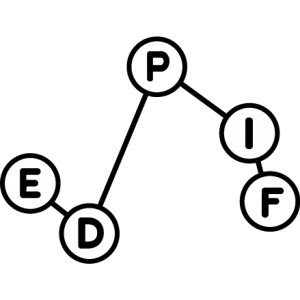
\includegraphics[height=0.7cm]{Figures/logo/EDPIF.png}\vspace{-0.5cm}}

%%%%%%%%%%%%%%%%%%%%%%%%%%%%%%%%%%%%%% Navigation symbols %%%%%%%%%%%%%%%%%%%%%%%%%%%%%%%%%%%%

\setbeamertemplate{navigation symbols}{}

% \setbeamertemplate{navigation symbols}{%
% 	\insertslidenavigationsymbol % Icône slide
% 	\insertframenavigationsymbol % Icône frame
% 	\insertsubsectionnavigationsymbol % Icône sous section
% 	\insertsectionnavigationsymbol % Icône section
% 	\insertdocnavigationsymbol % Icône docnavigation
% 	\insertbackfindforwardnavigationsymbol % Icône backfindforward
% }

%%%%%%%%%%%%%%%%%%%%%%%%%%%%%%%%%%%%%%%%%% Document %%%%%%%%%%%%%%%%%%%%%%%%%%%%%%%%%%%%%%%%%%

\begin{document}

	\begin{frame}[plain]
		\titlepage
	\end{frame}

    \section{Nitrogen fertilizers}
    \begin{frame}{}

        \centering
        \begin{tikzpicture}
            \node (image) [anchor=south west, inner sep=0pt] {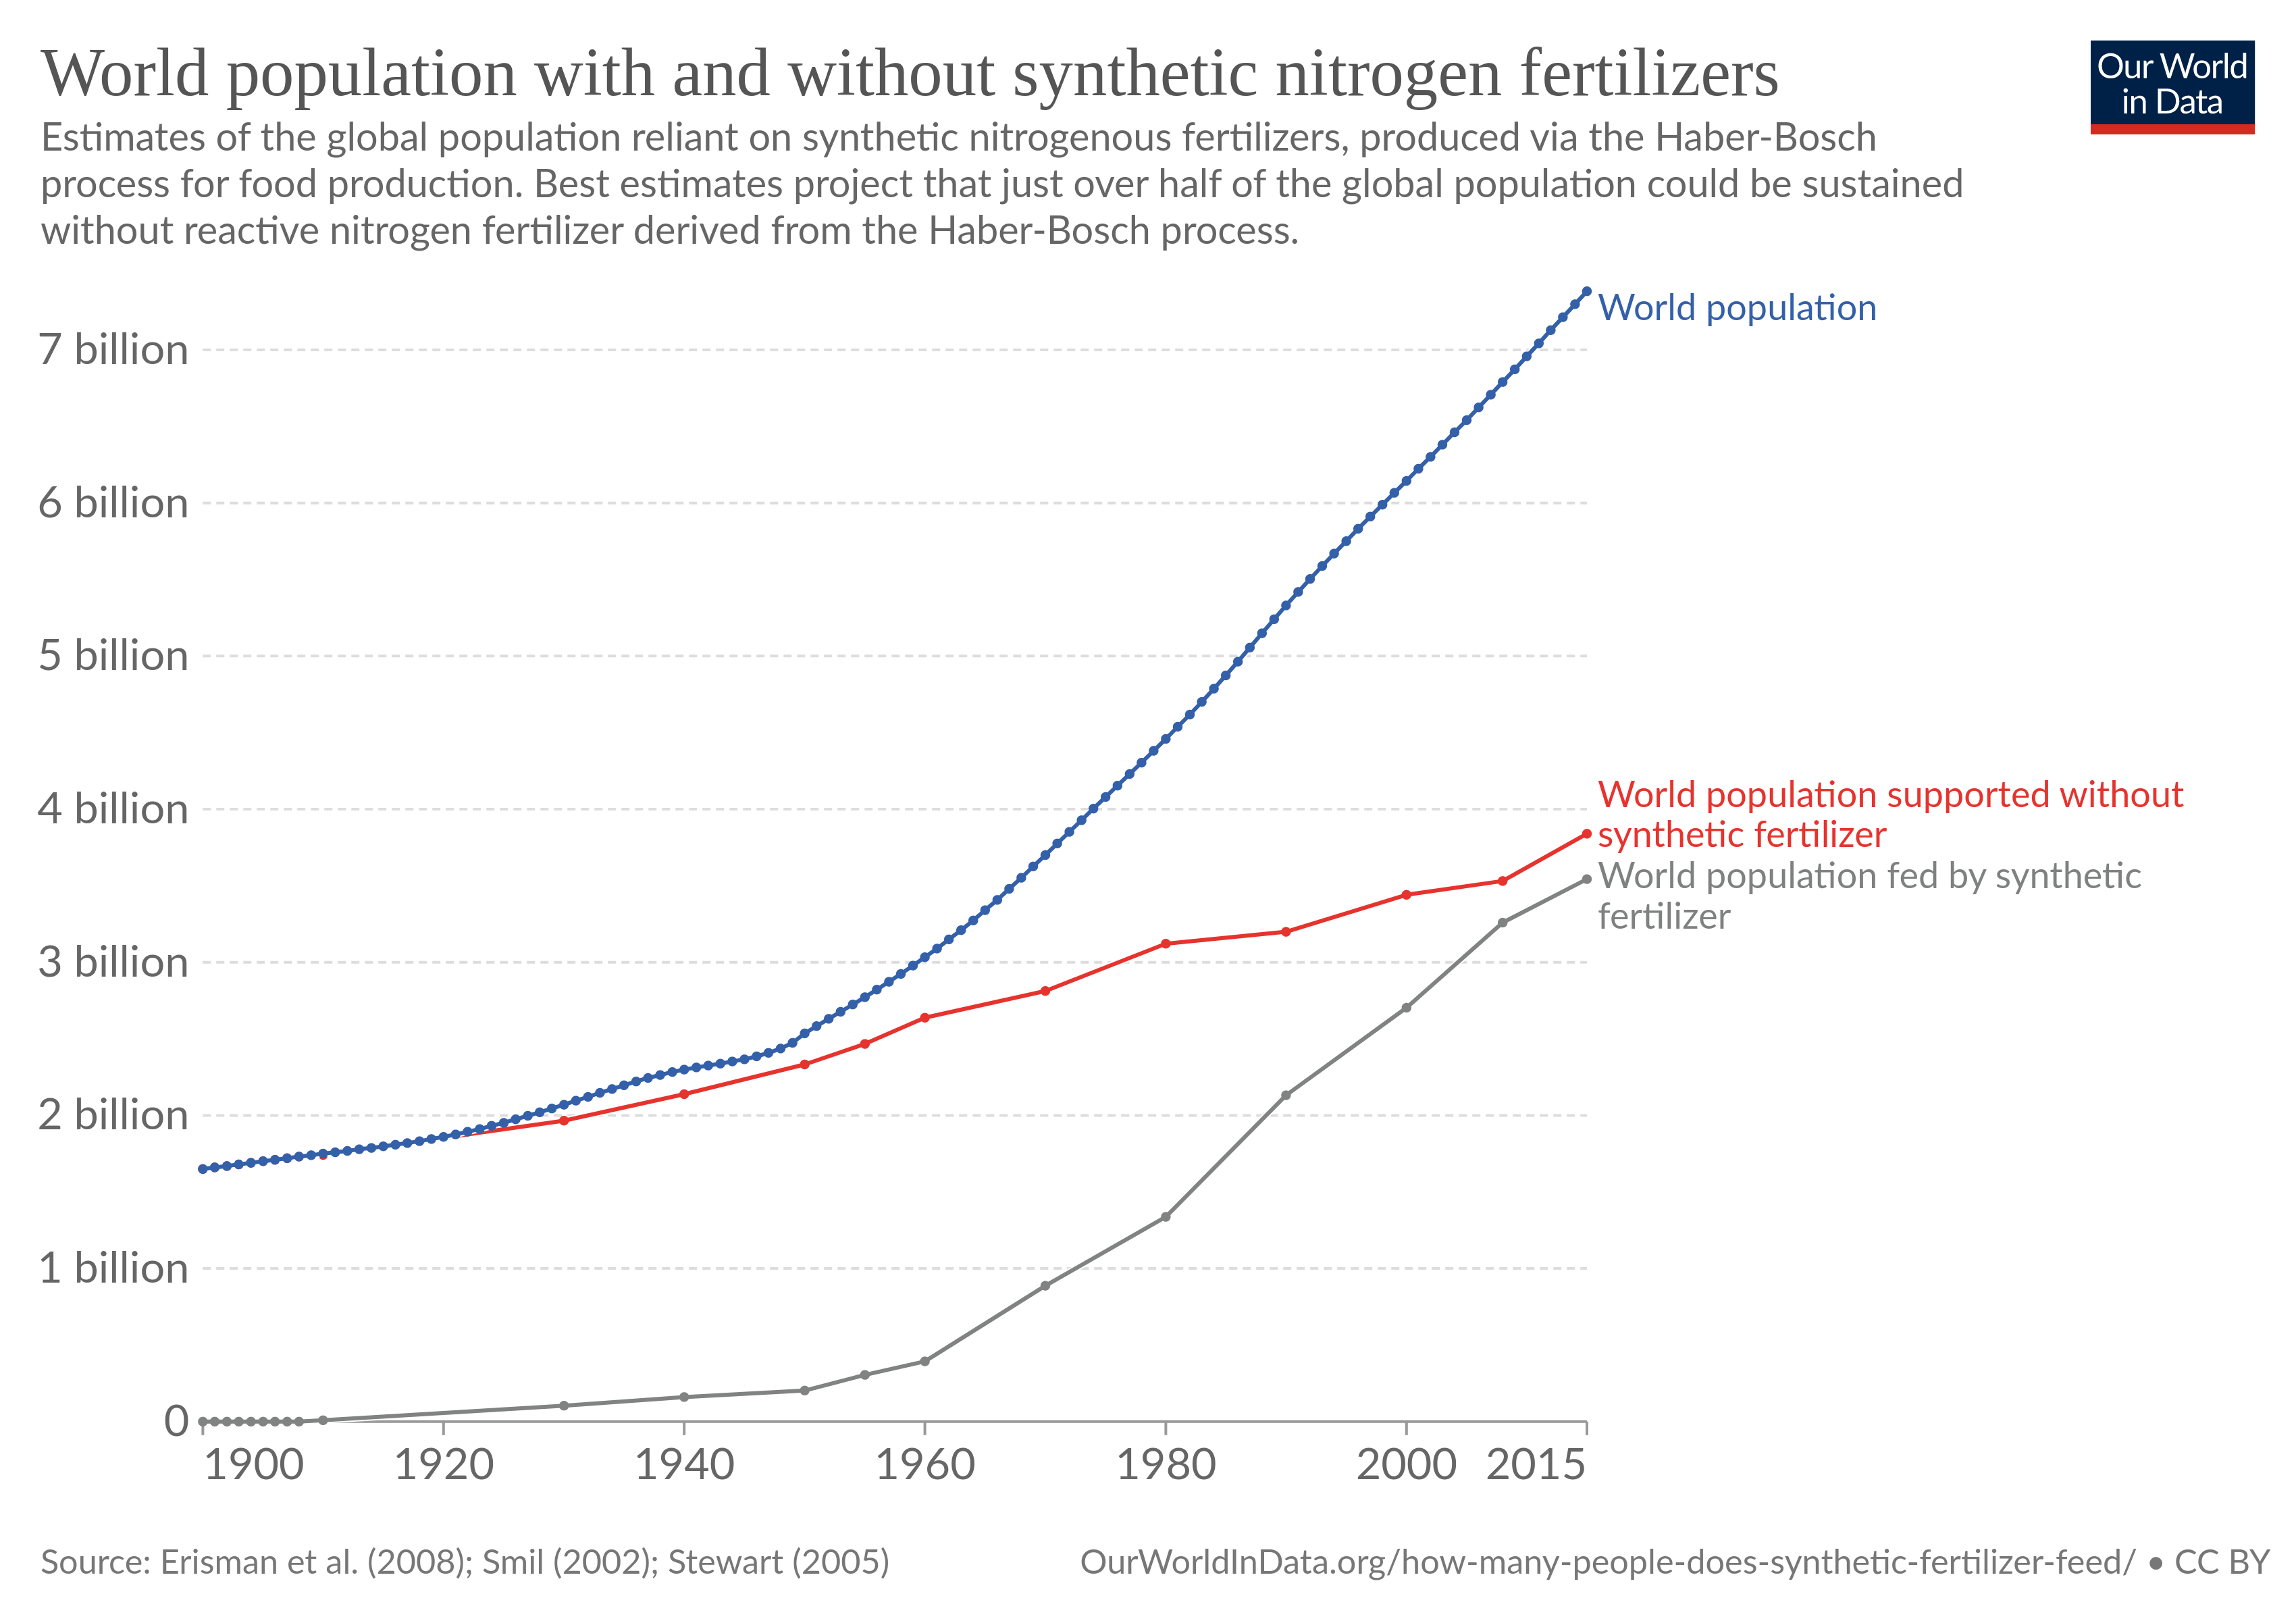
\includegraphics[width=0.99\textwidth]{Figures/worldindata/world-population-with-and-without-fertilizer.png}};
            \begin{scope}[x={(image.south east)}, y={(image.north west)}]
                \pause
                \node [text width=3cm,align=right] at (0.16, 0.7) (OP) {\textcolor{Ostwald}{Ostwald} process\\(1902)\\ \textrightarrow Nobel prize\\(1909)};
                \draw [-latex, ultra thick, Ostwald] (0.10,0.75) to (0.10,0.12);
                \pause
                \node [text width=3cm,align=right] at (0.18, 0.45) (HBP) {\textcolor{Haber}{Haber-Bosch}\\process (1908)\\ \textrightarrow Nobel prize\\(1918)};
                \draw [-latex, ultra thick, Haber] (0.13,0.4) to (0.13,0.12);
            \end{scope}
        \end{tikzpicture}
    
\end{frame}


    % \begin{frame}{}
    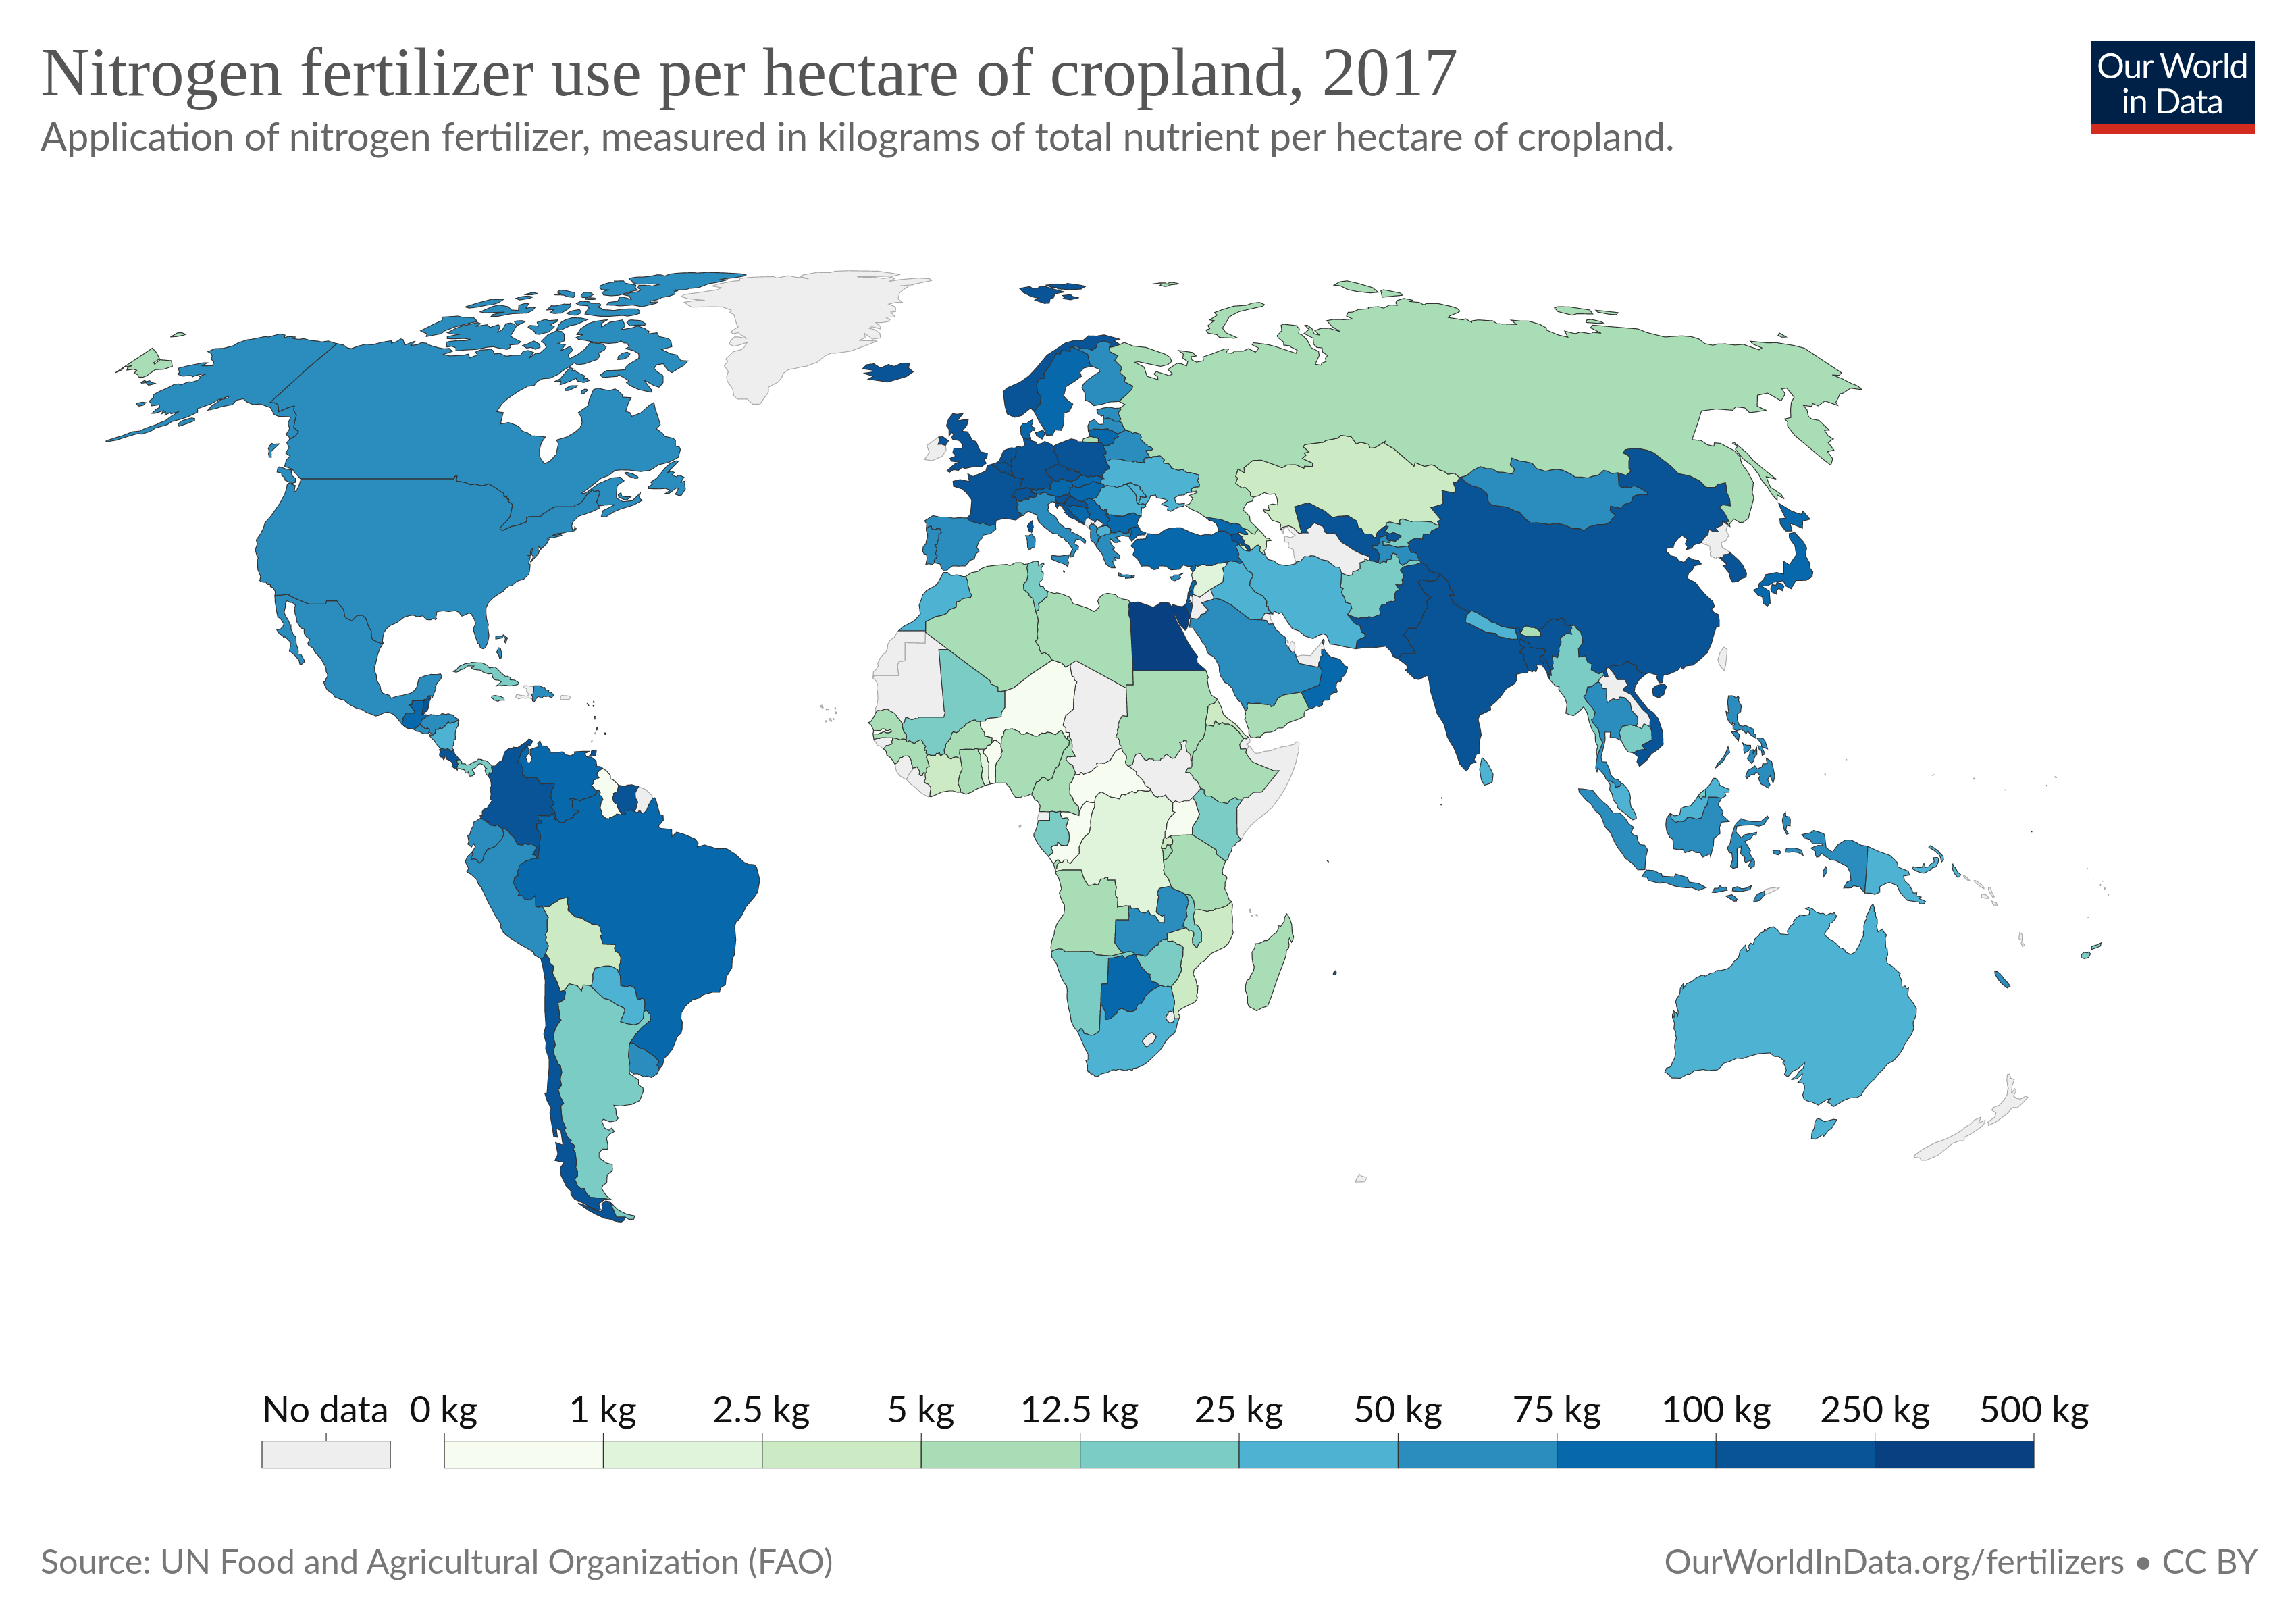
\includegraphics[width=0.99\textwidth]{Figures/worldindata/nitrogen-fertilizer-application-per-hectare-of-cropland.png}
\end{frame}
    \begin{frame}
    \frametitle{A high environmental and industrial impact}
    \medskip
    \begin{columns}

        \column[T]{0.35\textwidth}
            \centering 
            Stage 1
            \smallskip\\
            \small
            4 \ammonia + 3 \dioxygen → \ce{6 \water} + 2 \nitrogen\\
            4 \ammonia + 4 \dioxygen → \ce{6 \water} + 2 \nitrousoxide\\
            4 \ammonia + 5 \dioxygen → \ce{6 \water} + 4 \nitricoxide \\

            \bigskip
            \normalsize
            Stage 2
            \smallskip\\
            \small
            2\nitricoxide + \dioxygen → \ce{2 NO_2}\\
            \ce{3 NO_2 + H_2 O} → \nitricacid + \nitricoxide\\

            \bigskip
            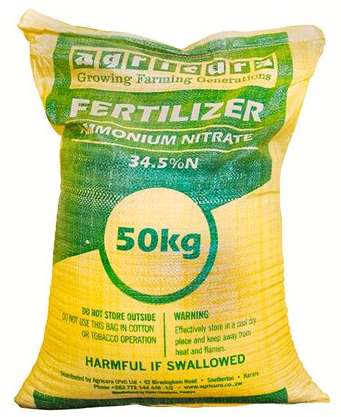
\includegraphics[width=0.6\textwidth]{Figures/ammonia/fertilizer.png}

        \column[T]{0.6\textwidth}
            \textcolor{Important}{{Ostwald process:}}
            \begin{enumerate}
                \item Producing \nitricoxide from \ammonia (Ammonia oxidation)
                \pause
                \item Producing \nitricacid from \nitricoxide
            \end{enumerate}

            \medskip
            \pause
            Why \nitricacid ?
            \begin{itemize}
                \pause
                \item Fertilizer synthesis: $\approx$ 60 million tonnes/year
                \pause
                \item TNT, mining industry
            \end{itemize}            

            \medskip
            \pause
            Other applications:
            \begin{itemize}
                \item Slip reaction, remove undesired \ammonia from industrial exhaust
                \pause
                \item Environmental reasons (\ammonia is a major air pollutant)
            \end{itemize}
            
            \medskip
            \color{Important}
                \pause
                Application → catalytic reaction tuned towards a specific product.\\
                \pause
                Selectivity → temperature, pressure, reactant ratio, type of catalyst.

            %connection between surface structure, and reaction conditions (e.g. feed composition, temperature) and catalytic activity and selectivity.
            
    \end{columns}    
\end{frame}
    \begin{frame}{Synchrotron techniques}

\begin{table}[]
    \centering
    \small
    \begin{tabular}{l|l|l|l}
        Technique & Sample & Sensitivity & Information \\
        \hline
        \hline
        \textcolor{Important}{Surface X-ray} & Pt monocrystals & Surface & Roughness, relaxation\\
        \textcolor{Important}{Diffraction (SXRD)} & (111), (100) & structure & and crystallographic phases \\
        % \hline
        % \pause
        % \textcolor{Blue}{X-ray Photoelectron}  & Pt monocrystals & Surface & Species presence, \\
        % \textcolor{Blue}{Spectroscopy (XPS)} & (111), (100) & species & quantity, oxidation state \\
        \hline
        % \pause
        \onslide<2->{\textcolor{Important}{Bragg Coherent}} & \onslide<2->{Pt nanoparticles} & \onslide<2->{Bragg electronic} & \onslide<2->{Shape, 3D strain}  \\
        \onslide<2->{\textcolor{Important}{Diffraction Imaging}} & \onslide<2->{(111), (110), (100), ...} & \onslide<2->{density} & \onslide<2->{and displacement arrays} \\
        \onslide<2->{\textcolor{Important}{(BCDI)}} & \onslide<2->{} & \onslide<2->{} & \onslide<2->{}\\
    \end{tabular}
    \caption{Near-ambient pressure (NAP) X-ray techniques carried out at \textcolor{Important}{SixS} (SOLEIL).}% or \textcolor{Blue}{B-07} (Diamond) synchrotrons for the present study.}
    \label{tab:techniques}
\end{table}

\vspace{-0.5cm}

% \begin{figure}
% \centering
    % \onslide<2->{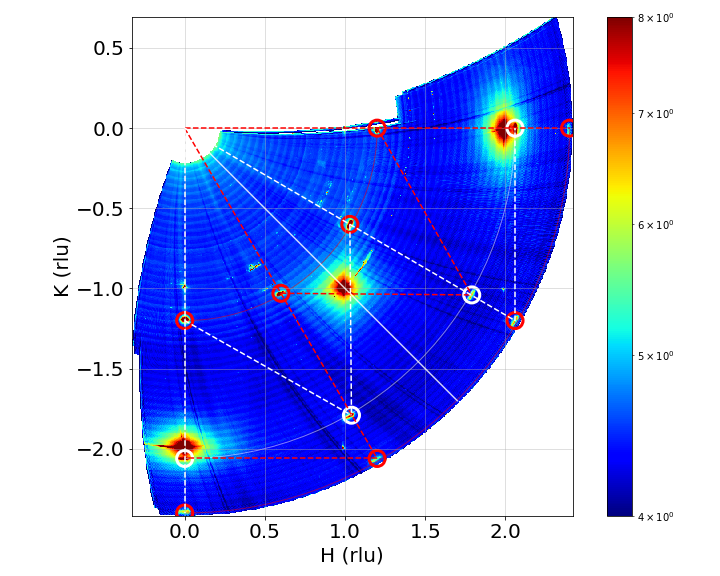
\includegraphics[width=0.45\textwidth]{Figures/sxrd_data/maps/Map_hkl_surf_or_2227-2283.png}}
    %%%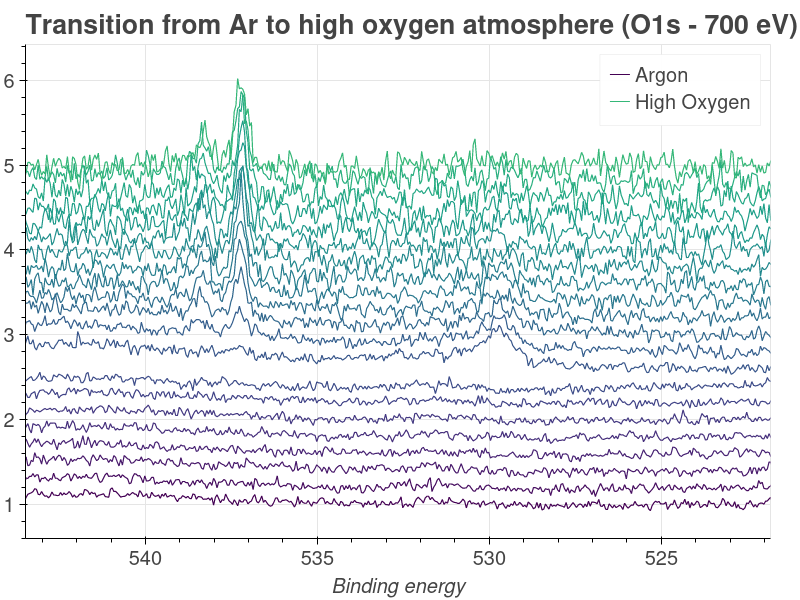
\includegraphics[width=0.32\textwidth]{Figures/xps_data/transition_xps.png}
    %%% 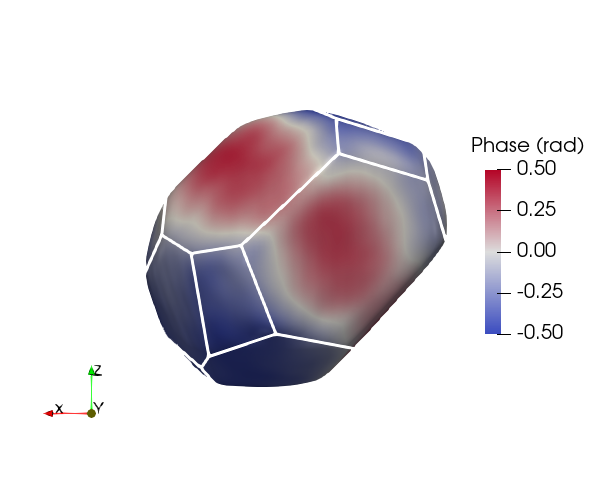
\includegraphics[width=0.42\textwidth]{Figures/gwaihir/facets_D6.png}
    % \onslide<2->{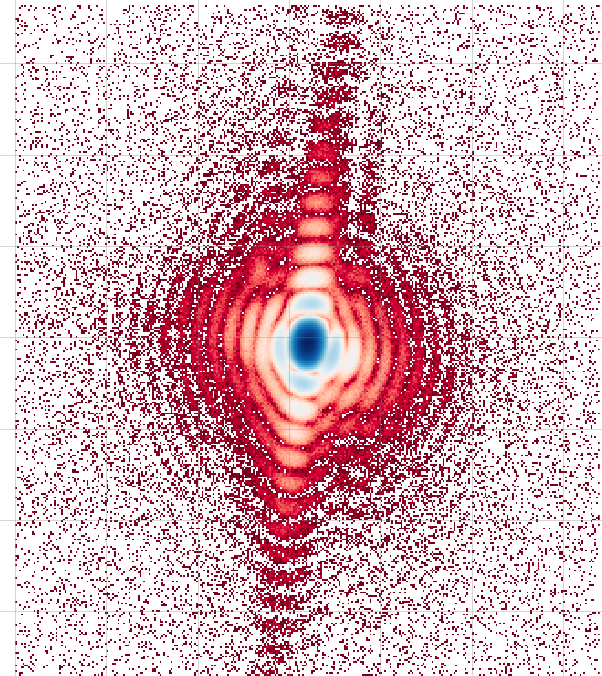
\includegraphics[width=0.35\textwidth]{Figures/gwaihir/dp_pr.png}}
% \end{figure}

\begin{center}
\hspace{-0.5cm}
    {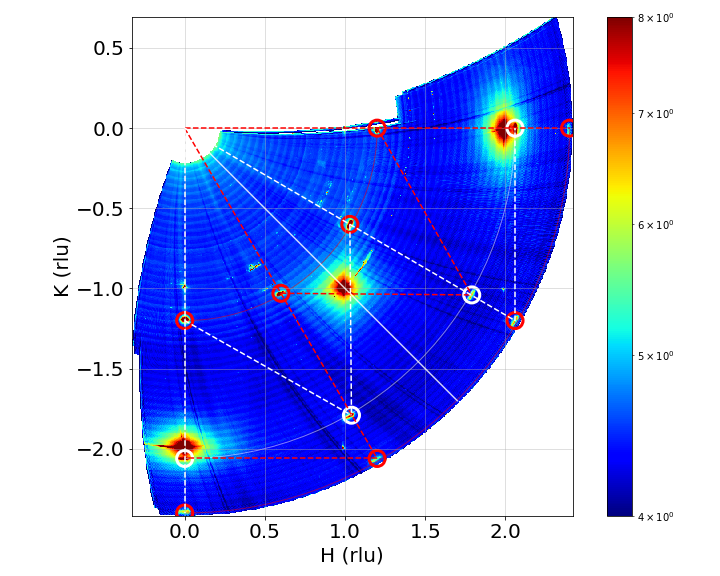
\includegraphics[height=0.55\textheight]{Figures/sxrd_data/maps/Map_hkl_surf_or_2227-2283.png}}
    \onslide<2->{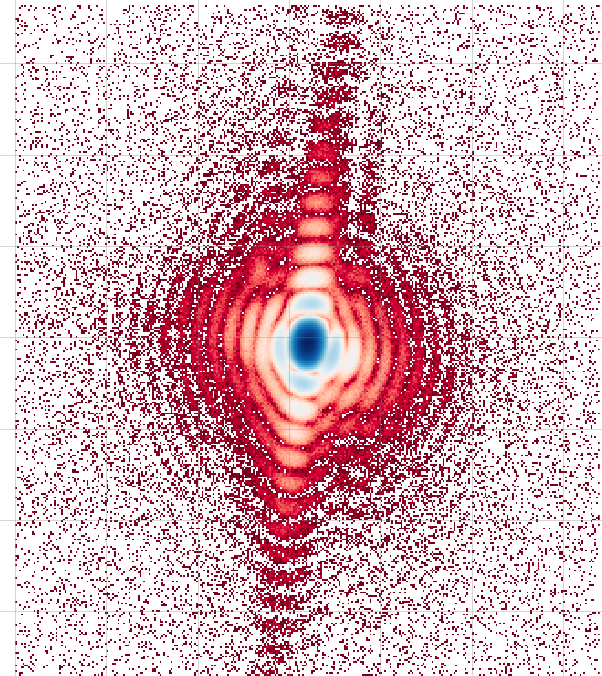
\includegraphics[height=0.55\textheight]{Figures/gwaihir/dp_pr.png}}
\end{center}    
    
\end{frame}

    % \section{Literature review}
    % \begin{frame}{Pt 100}

Structure on Blender
    
\end{frame}
    % \begin{frame}{Pt 111}
    
\end{frame}
    
	\section{Experimental setup}
    \begin{frame}{Sample environment at SixS}

    \begin{columns}
    
        \column[T]{0.62\textwidth}
            \begin{figure}
                \centering
                \captionsetup{width=\textwidth}
                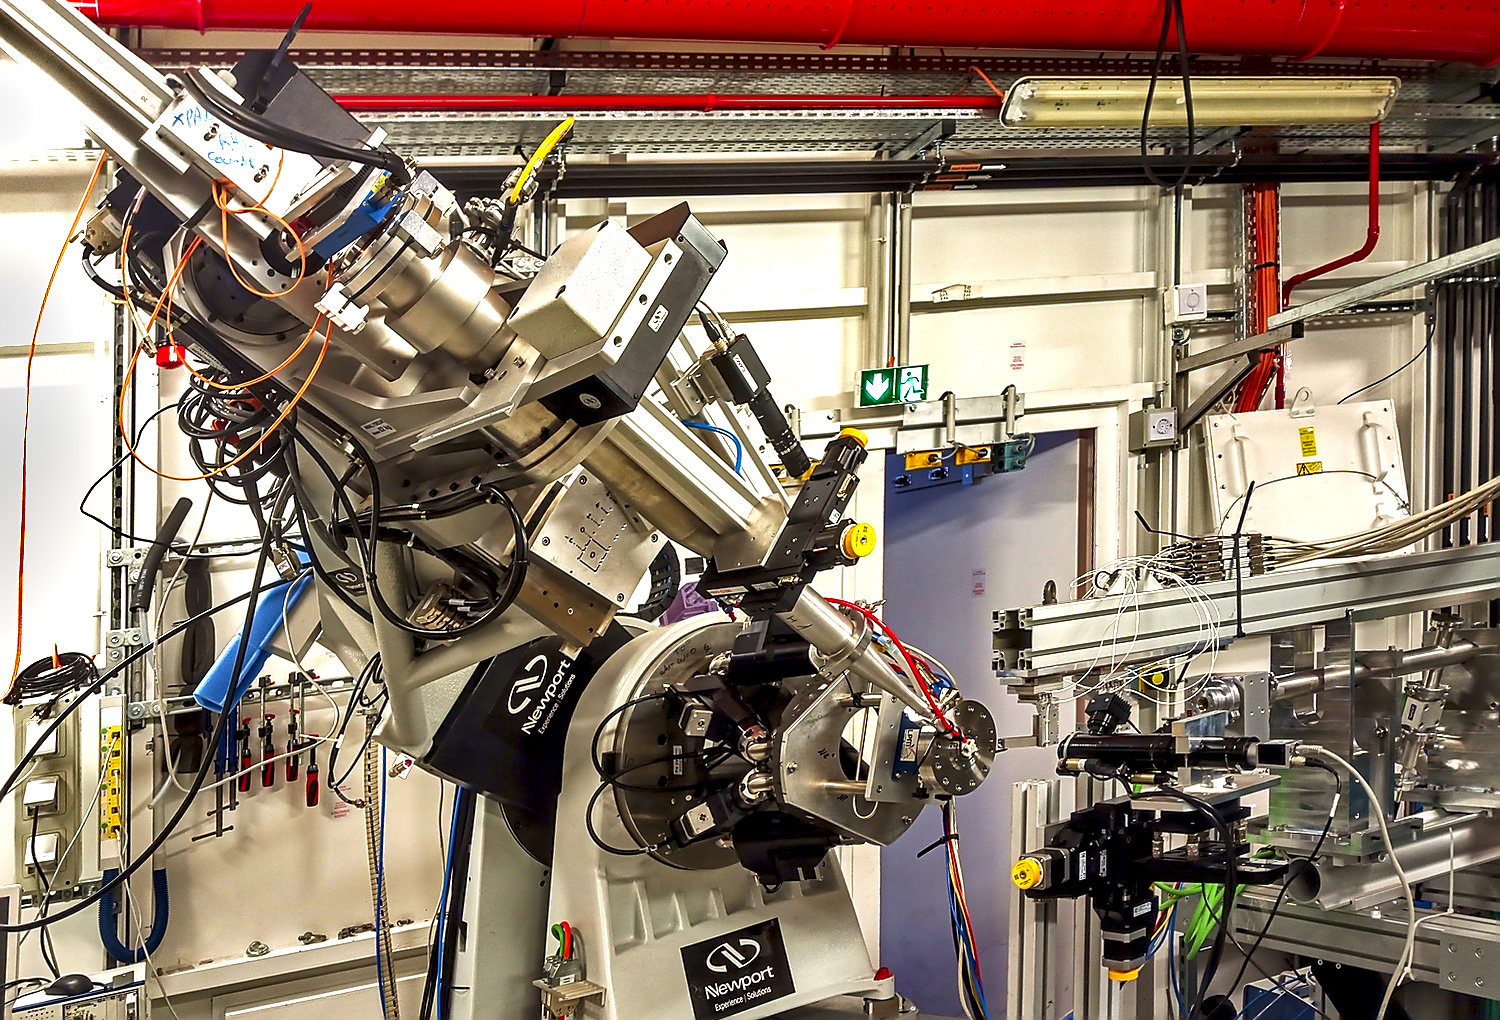
\includegraphics[width=\textwidth]{Figures/sixs/MED.jpg}
                \caption{Multi Environment Diffractometer (MED), experimental end station at SixS}
                \label{fig:MED}
            \end{figure}

            → Study ammonia oxidation

        \column[T]{0.32\textwidth}
            \pause
            \begin{figure}
                \centering
                \captionsetup{width=\textwidth}
                \includegraphics[width=\textwidth]{Figures/sixs/CELL.jpg}
                \caption{XCAT reactor cell and dome for NAP and AP experiments}
                \label{fig:XCAT}
            \end{figure}

            \begin{itemize}
                \pause
                \item Gas panel with mass flow controllers (Argon, \ammonia, \dioxygen, …)
                \pause
                \item Sample heater
                \pause
                \item Mass spectrometer: residual gas analyser (RGA)
            \end{itemize}
            
    \end{columns}
\end{frame}
    \begin{frame}{Conditions}
    \bigskip
    \setlength{\arrayrulewidth}{0.2mm}
    \setlength{\tabcolsep}{08pt} % padding on sides
    \renewcommand{\arraystretch}{1.2} % height

    \centering
    \small
    \begin{tabular}{ |p{4cm}|p{1.5cm}|p{1.5cm}|p{1.5cm}| }
        \hline
        Gas flow (constant: $50$ mL/min, $0.3$ bar) & RT & \textcolor{Important}{300°C} & \textcolor{Important}{400°C} \\
        \hline
        Argon (inert gas) & \multicolumn{3}{l|}{Catalyst state without reactants (unactive)}\\ \hline
        1 \ammonia & \multicolumn{3}{l|}{NH3 introduction influence}\\ 
        \hline
        1 \ammonia + 0.5 \dioxygen & \multicolumn{3}{c|}{}\\
        1 \ammonia + 1 \dioxygen & \multicolumn{3}{c|}{\multirow{-2}{*}{Influence of \ammonia / \dioxygen ratio as a function}}\\
        1 \ammonia + 2 \dioxygen & \multicolumn{3}{c|}{\multirow{-2}{*}{of the temperature and vice-versa}}\\
        1 \ammonia + 8 \dioxygen & \multicolumn{3}{c|}{} \\ 
        \hline
    \end{tabular}

    \pause
    \begin{figure}
        \centering
        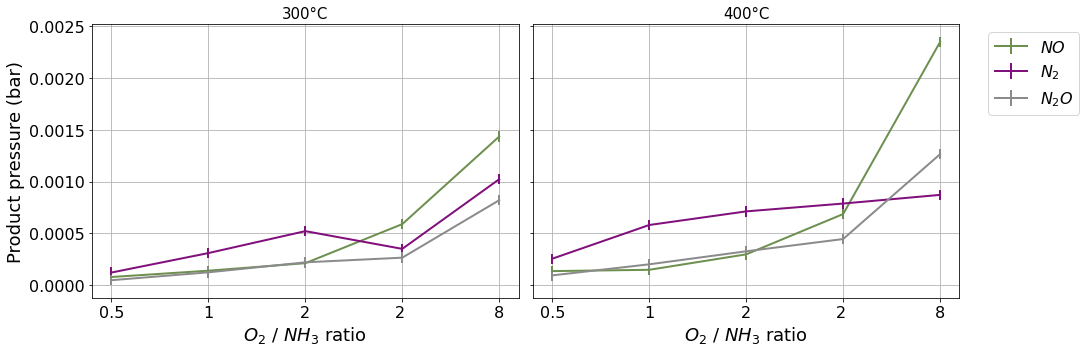
\includegraphics[width=0.9\textwidth]{Figures/sxrd_data/rga/product_comparison.png}
        \label{fig:product_pressure}
        \caption{Product pressure evolution with temperature and input gas}
    \end{figure}
    
\end{frame}
    \begin{frame}{Why develop BCDI at SixS}
    \begin{columns}
        \column[T]{0.65\textwidth}
            \begin{itemize}
                \item Complementary with Surface X-Ray Diffraction \pause
                \item Same reactor cell allowing \textit{in-situ} and \textit{operando} experiments at ambient pressure followed with a mass spectrometer
            \end{itemize}
            \pause 
            
            \begin{figure}
                \centering
                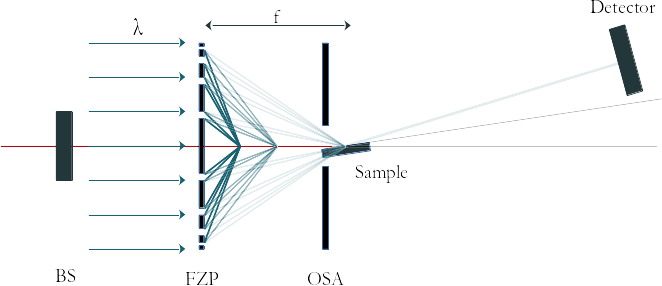
\includegraphics[width=\textwidth]{Figures/sixs/optical_setup.png}
                \caption{Optical elements improve the coherent flux on the sample.}
                \label{fig:optical_setup}
            \end{figure}
            \pause

            \begin{tabular}{l|l|l|l|l}
                 & Beam stop & FZP & OSA & Beam\\ \hfill
                Diameter $\Omega$ & $80 \, \mu m$ & $300 \, \mu m$ & $70 \, \mu m$ & $\approx 1 \, \mu m$\\
            \end{tabular}
            \pause

        \column{0.3\textwidth}
            \begin{figure}
                \centering
                \includegraphics[width=\textwidth]{Figures/sixs/CELL.jpg}
                \caption{Reactor cell and dome}
                \label{fig:CELLDome}
                \bigskip
                \pause
                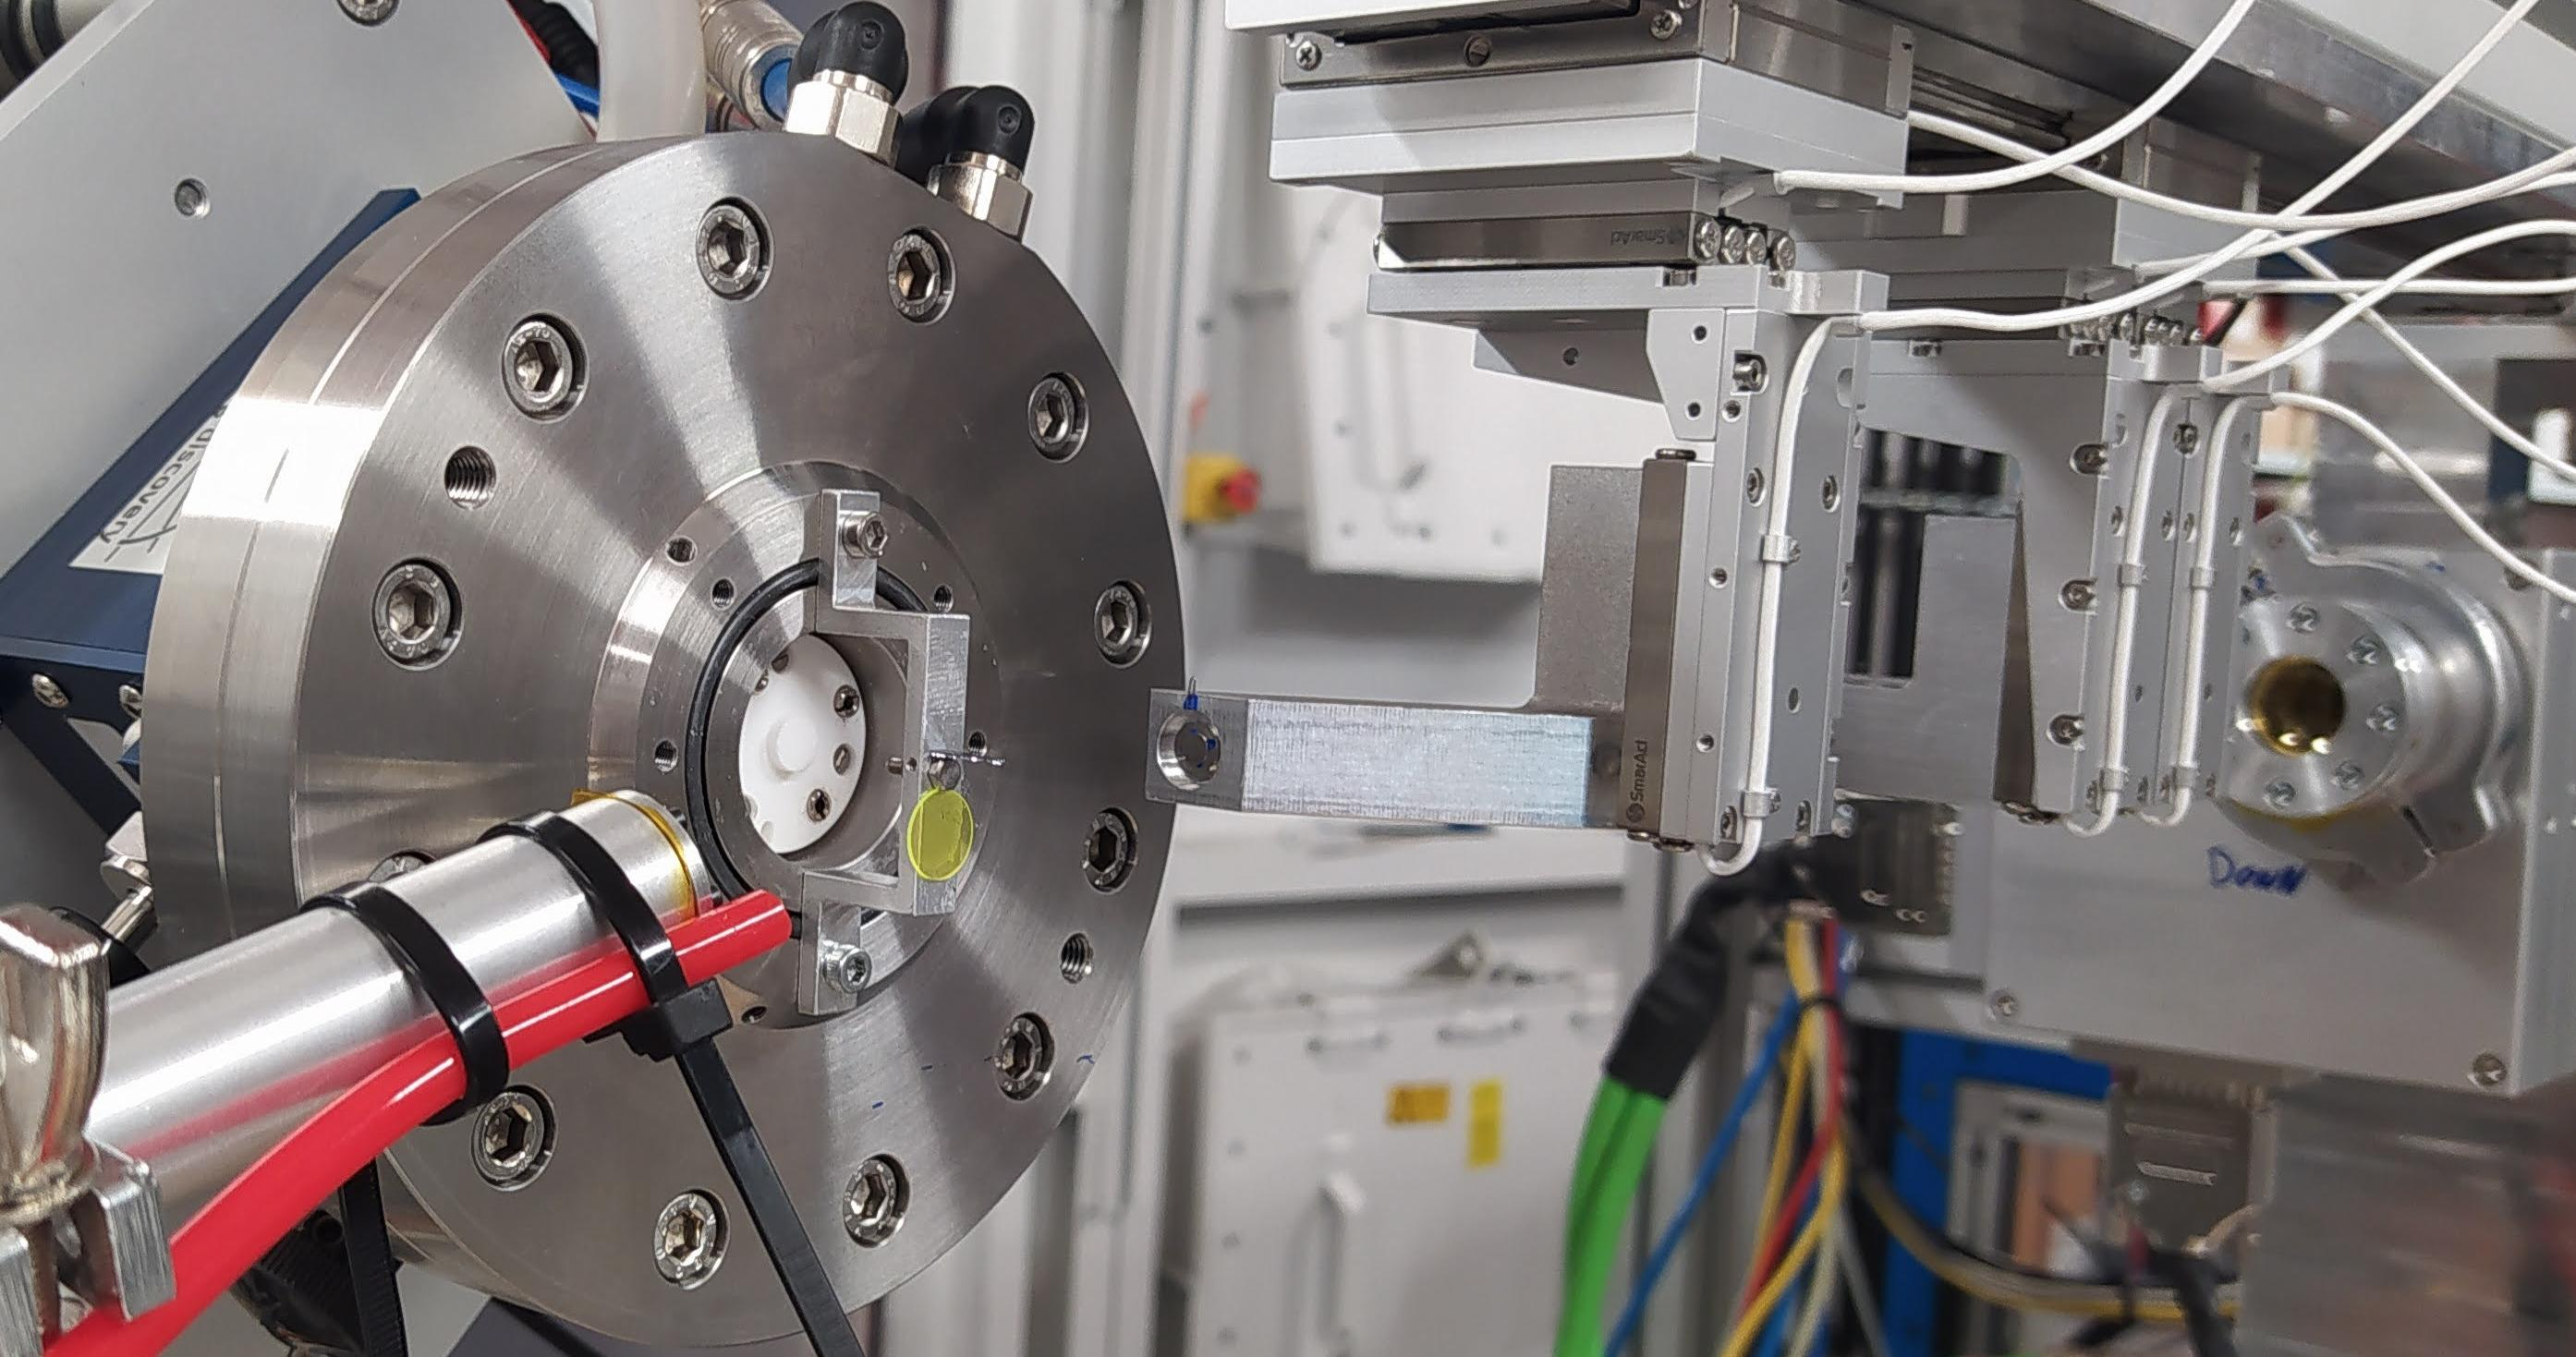
\includegraphics[width=\textwidth]{Figures/sixs/opt_elements_photo.jpg}
                \caption{Coherence slits → beam stop (BS) → Fresnel zone plates (FZP) → order selecting aperture (OSA) → XCAT reactor}
                \label{fig:3Doptics}
            \end{figure}

    \end{columns}
\end{frame}
    \begin{frame}{Catalyst sample: Pt nanoparticles}
    \medskip
    \begin{columns}

        \column[T]{0.45\textwidth}
    
            Patterned sample:
            \begin{itemize}
                \item Dewetted (111)-oriented nanoparticles
                \item (001)-oriented sapphire ($\alpha$-\ce{Al_2O_3}) substrate
                \item 24 hours annealed in air @1100°C
                %\item Model catalyst, similar to Pt foils
                % Wickham, D.T., B.A. Banse, and B.E. Koel, The adsorption of nitric oxide and nitrogen dioxide on polycrystalline platinum. Surf. Sci., 1989. 223: p. 82-100.
            \end{itemize}

            \vspace{0.5cm}
            \begin{figure}
                \centering
                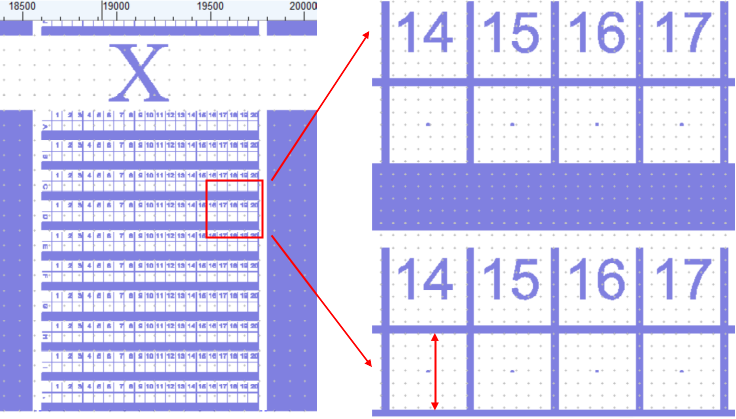
\includegraphics[width=\textwidth]{Figures/sample/mask.png}
                \caption{Mask during sample preparation (area in blue)}
                \label{fig:mask}
            \end{figure}

        \pause
        \column[T]{0.5\textwidth}

            \begin{figure}
                \centering %left bottom right top
                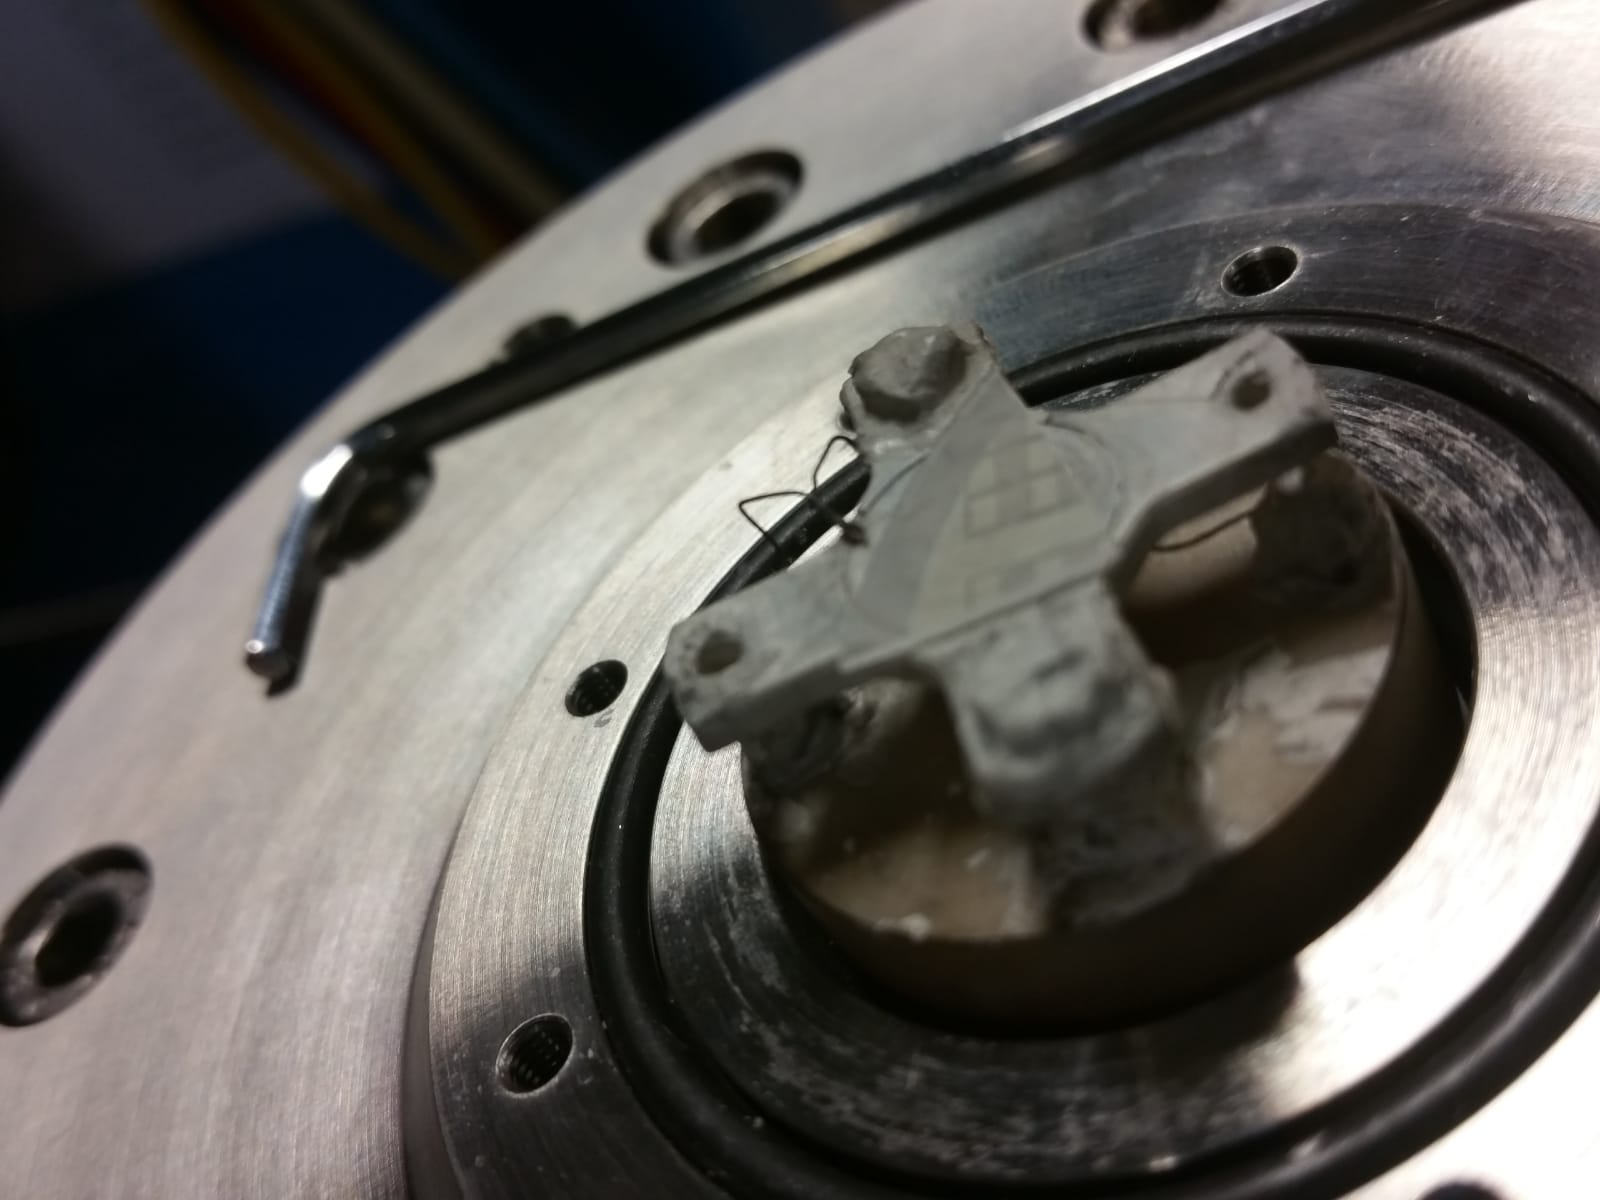
\includegraphics[trim=650 300 250 250, clip, width=0.45\textwidth]{Figures/sample/reactor_cell.jpeg}
                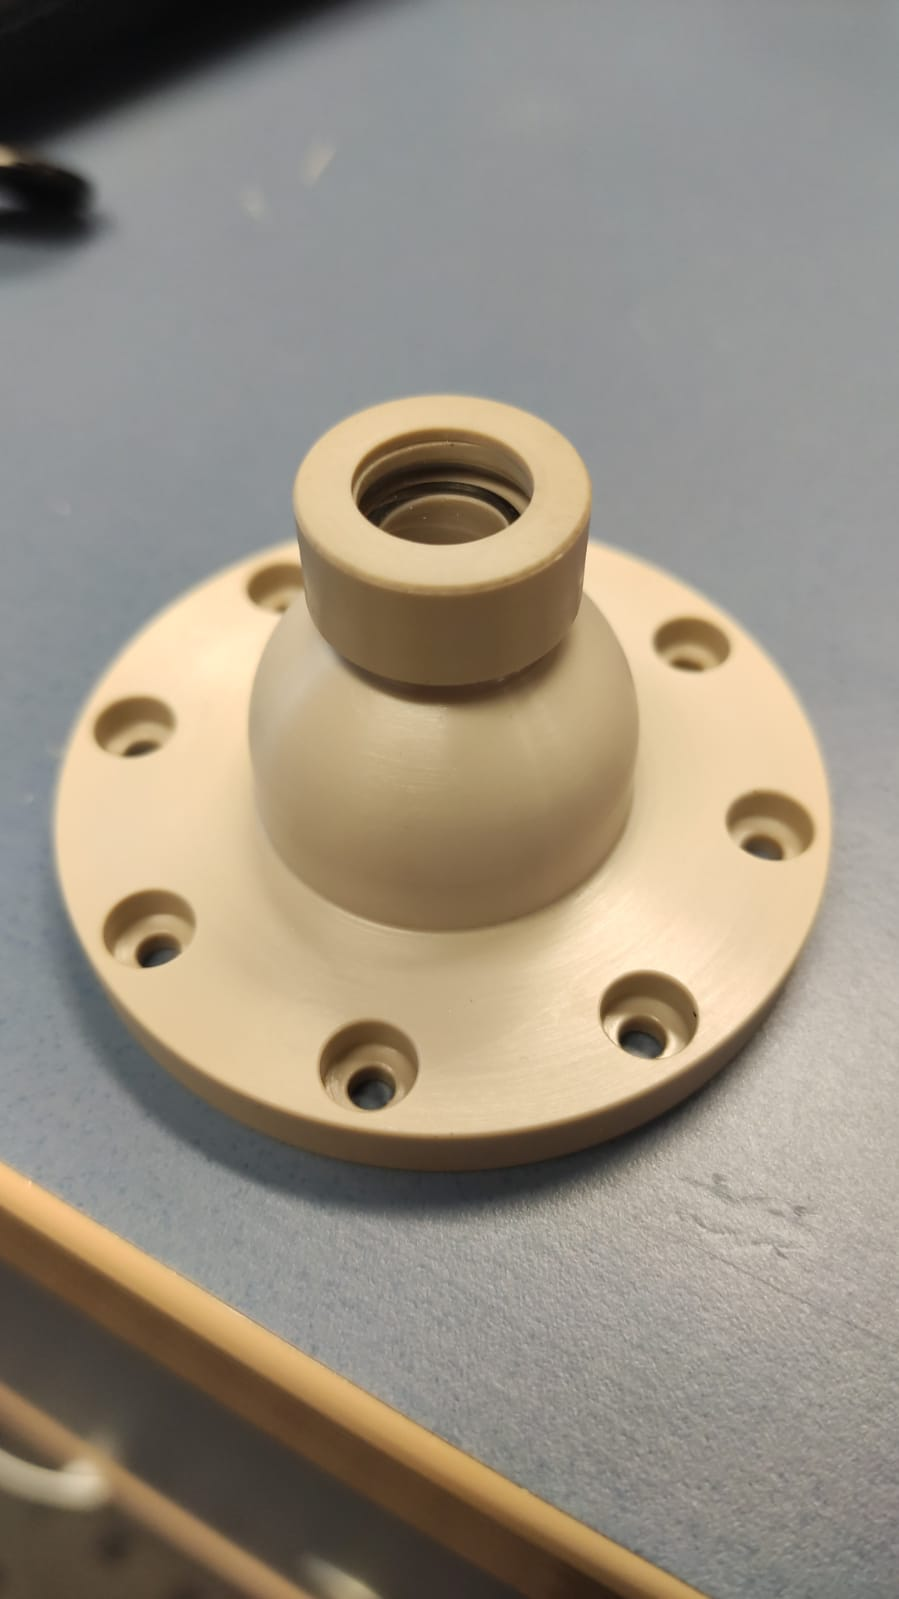
\includegraphics[trim=0 400 0 380, clip, width=0.45\textwidth]{Figures/sixs/dome_window.png}
                \caption{Sample holder, paste in Boron Nitride, wafer in Sapphire.}
                \label{fig:sample_and_dome}
            \end{figure}

            \pause
            
            \begin{figure}
                \centering %left bottom right top
                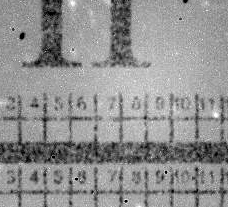
\includegraphics[trim=0 0 0 10, clip, width=0.45\textwidth]{Figures/sample/microscope_image.png}
                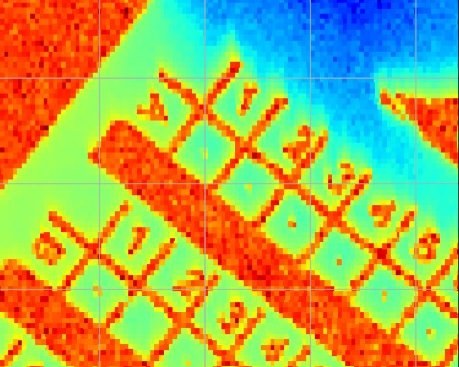
\includegraphics[width=0.45\textwidth]{Figures/sample/microscope_image_photon.png}
                \caption{Microscope image}
                \label{fig:microscope_image}
            \end{figure}
    \end{columns}

\end{frame}
    \begin{frame}{How to measure 3D diffraction patterns at SixS ?}
    \begin{columns}
        \column[T]{0.45\textwidth}
        \begin{figure}
            \centering
            \begin{tikzpicture}
                \node (image) [anchor=south west, inner sep=0pt] {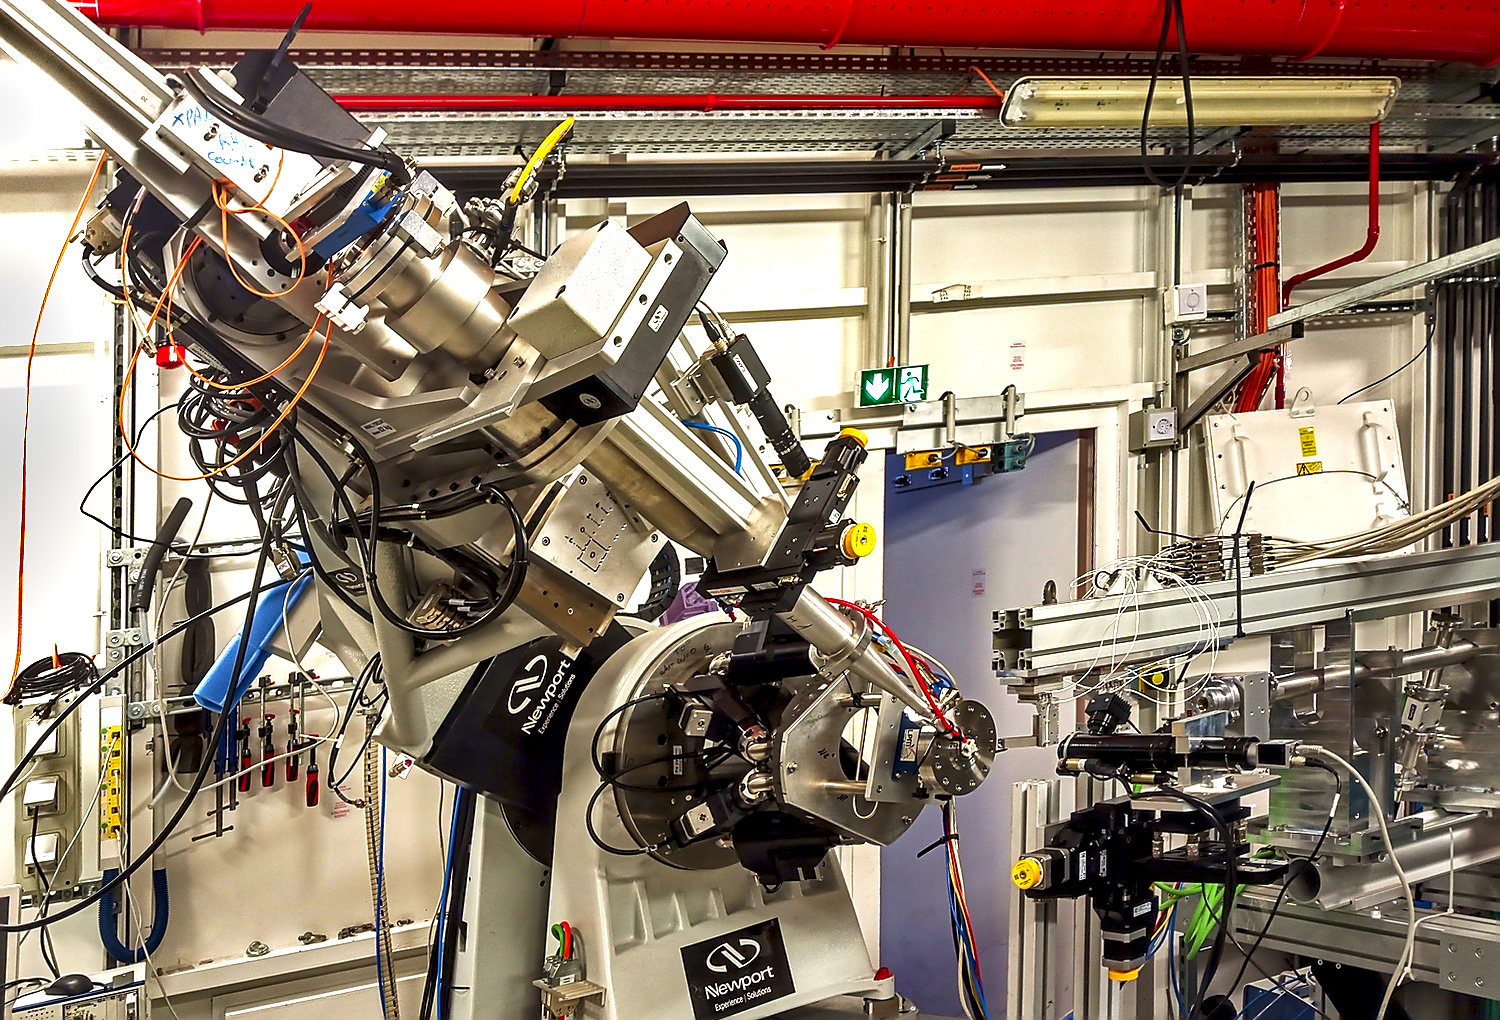
\includegraphics[trim=0 30 100 20, clip, width=\textwidth]{Figures/sixs/MED.jpg}};
                \begin{scope}[x={(image.south east)}, y={(image.north west)}]
                    \node [fill=white,rounded corners=2pt,inner sep=1pt] at (0.7,0.2) {Sample};
                    \node [fill=white,rounded corners=2pt,inner sep=1pt] at (0.35,0.7) {Detector};
                \end{scope}
            \end{tikzpicture}
            \caption{Multi Environment Diffractometer (MED), experimental end station at SixS}
            \label{fig:MED_3D}
        \end{figure}
        
        \vspace{-0.4cm}
        
        \begin{gather*}
            I(\vec{q}_{hkl}) \propto ||F(\vec{q}_{hkl})||^2\\
            F(\vec{q}_{hkl}) = \sum_j^N f_j (\vec{q}_{hkl}) \exp^{i(\vec{q}_{hkl}.\vec{u}(\vec{r}))}
        \end{gather*}

        \column[T]{0.45\textwidth}
        
    \end{columns}
    
\end{frame}


\begin{frame}{How to measure 3D diffraction patterns at SixS ?}
    \begin{columns}
        \column[T]{0.45\textwidth}
        \begin{figure}
            \centering
            \begin{tikzpicture}
                \node (image) [anchor=south west, inner sep=0pt] {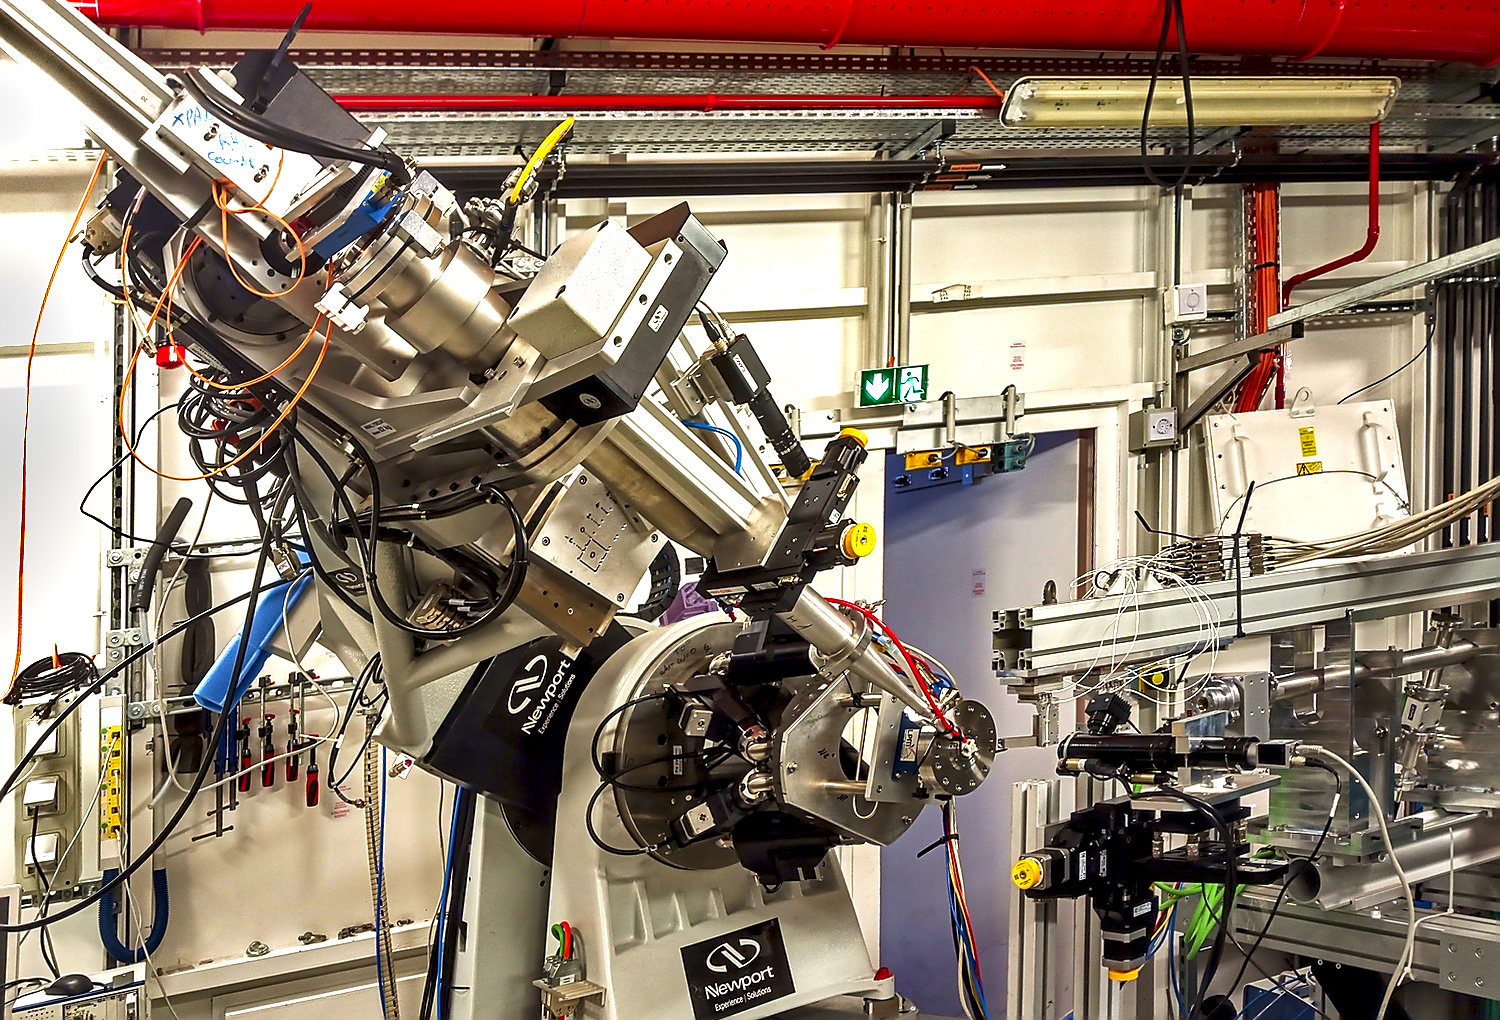
\includegraphics[trim=0 30 100 20, clip, width=\textwidth]{Figures/sixs/MED.jpg}};
                \begin{scope}[x={(image.south east)}, y={(image.north west)}]
                    \node [fill=white,rounded corners=2pt,inner sep=1pt] at (0.7,0.2) {Sample};
                    \node [fill=white,rounded corners=2pt,inner sep=1pt] at (0.35,0.7) {Detector};
                \end{scope}
            \end{tikzpicture}
            \caption{Multi Environment Diffractometer (MED), experimental end station at SixS}
        \end{figure}
        
        \vspace{-0.4cm}
        
        \begin{gather*}
            I(\vec{q}_{hkl}) \propto ||F(\vec{q}_{hkl})||^2\\
            F(\vec{q}_{hkl}) = \sum_j^N f_j (\vec{q}_{hkl}) \exp^{i(\vec{q}_{hkl}.\vec{u}(\vec{r}))}
        \end{gather*}

        \column[T]{0.45\textwidth}
        
        \begin{figure}
            \centering
            \animategraphics[trim=200 0 200 0, autoplay,loop, clip, width=0.9\textwidth]{5}{Figures/bcdi_data/3D_DP/DP_white_}{1}{20}
            \caption{Coherent fringes visible in multiple directions in 3D diffraction pattern}
        \end{figure}
    \end{columns}
    
\end{frame}

    \section{Gwaihir}
    \begin{frame}{Phase retrieval}
    \begin{columns}

        \column[T]{0.58\textwidth}
        \begin{figure}
            \centering
            \animategraphics[width=\textwidth,autoplay,loop]{1}{Figures/gwaihir/animated_pr/merged_image_}{1}{10}
            \caption{Phase retrieval with PyNX using iterative algorithms. \footnotemark}
            \label{fig:pr_pynx}
        \end{figure}

        Bragg electronic density:
        \begin{equation*}
            \rho_{crystal}(\Vec{r}) \exp^{i(\Vec{q}_{hkl}.\Vec{u}
            (\Vec{r}))}
        \end{equation*}

        \column[T]{0.38\textwidth}
    
        \begin{figure}
            \centering
            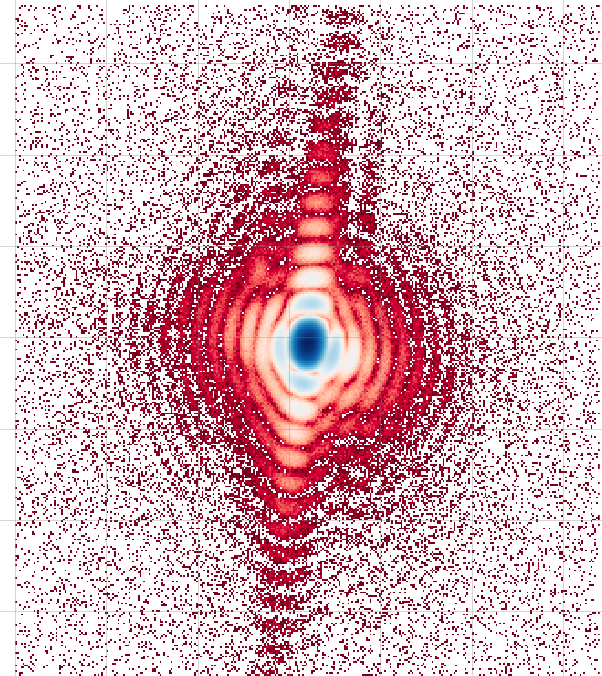
\includegraphics[width=0.8\textwidth]{Figures/gwaihir/dp_pr.png}
            \pause
            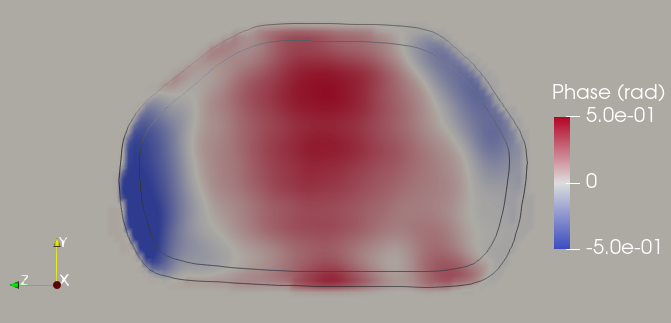
\includegraphics[width=0.8\textwidth]{Figures/gwaihir/obj_pr.png}
            \caption{Bragg peak (top) and reconstructed particle (bottom).}
            \label{fig:pr_dp_particle}
        \end{figure}

    \end{columns}

    \footnotetext{Favre-Nicolin, V., et al  (2011). Journal of Applied Crystallography, 44(3), 635–640.}
\end{frame}


    
    \begin{frame}{BCDI data analysis workflow}
    \begin{columns}
        \column[T]{0.48\textwidth}
        \begin{figure}
            \centering
            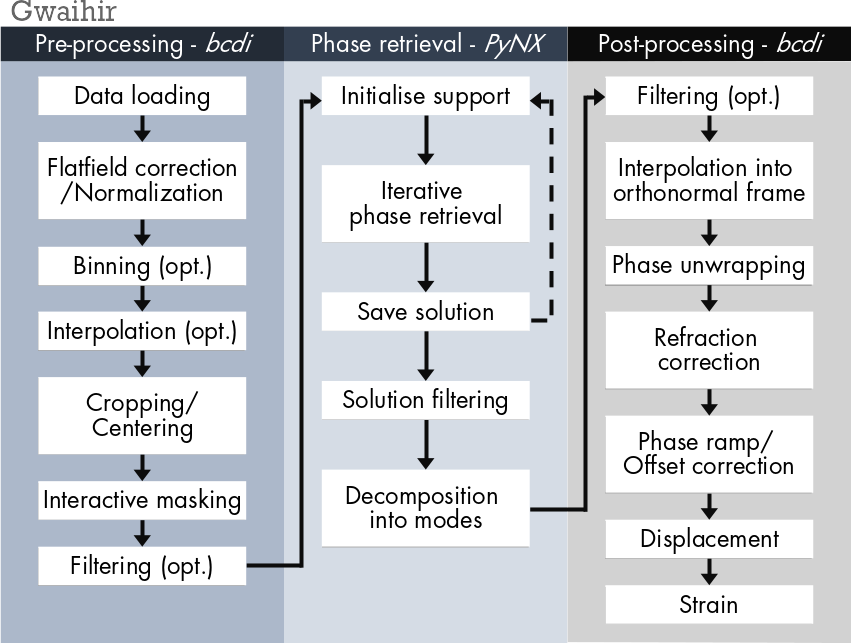
\includegraphics[width=\textwidth]{Figures/gwaihir/Packages.png}
            \caption{Flow chart of the main steps in the BCDI data analysis workflow.}
            \label{fig:Packages}
        \end{figure}
        
        \column[T]{0.48\textwidth}

        \pause
        
        \begin{figure}
            \centering
            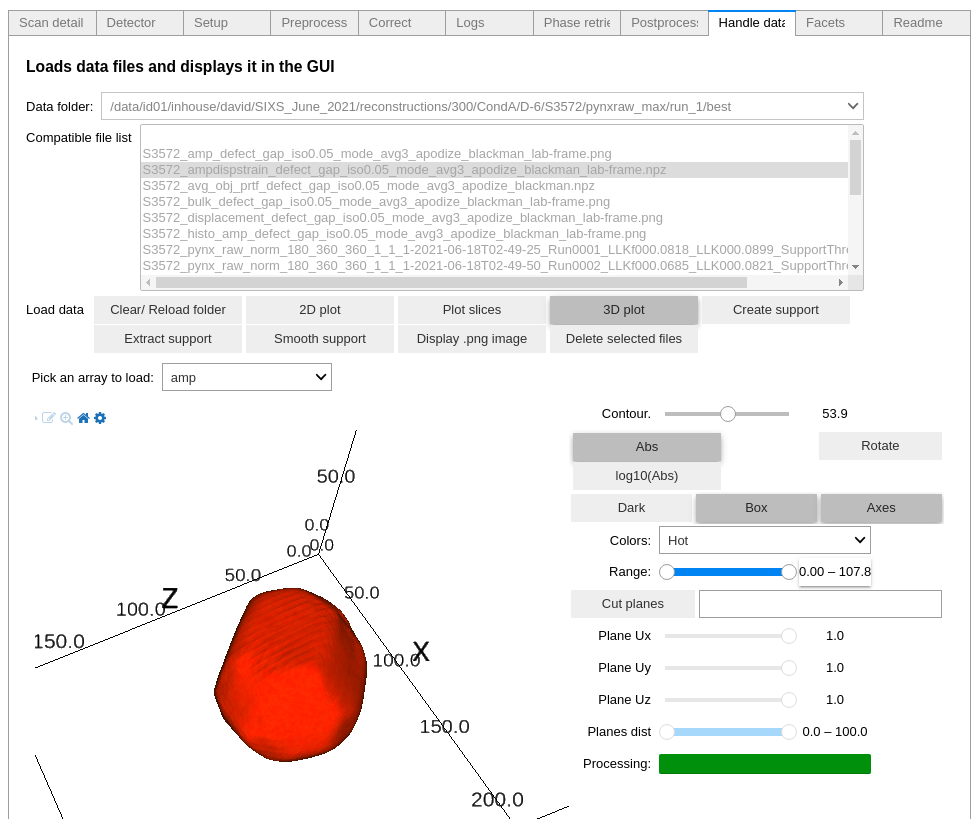
\includegraphics[width=\textwidth]{Figures/gwaihir/GUI_handle_tab.png}
            \caption{Data analysis is performed through interactive widgets.}
            \label{fig:GUI_handle_tab}
        \end{figure}

    \end{columns}

    \pause
    \begin{columns}
        \column[T]{0.03\textwidth}
        \vspace{-0.02cm}
        \begin{figure}[T]
            
\includegraphics[width=\textwidth]{Figures/gwaihir/GitHub-Mark-120px-plus.png}
        \end{figure}
        
        \column[T]{0.9\textwidth}
        \medskip
        GitHub repository (open access\footnotemark{}): \href{GitHub.com/Dsimonne/Gwaihir\#welcome}{GitHub.com/Dsimonne/Gwaihir\#welcome}
        
    \end{columns}
    
    \footnotetext{Gwaihir: Jupyter Notebook Graphical User Interface for Bragg Coherent Diffraction Imaging D. Simonne et al., (2022). J. Applied Crystallography (Volume 55, Part 4)}
\end{frame}

    \section{Bragg Coherent Diffraction Imaging}
    \begin{frame}{Facets on Pt nanoparticles}
    \begin{columns}
        \column[T]{0.45\textwidth}
        \centering
        A: $\diameter \approx 800 nm$ 
        \begin{figure}
            \centering
            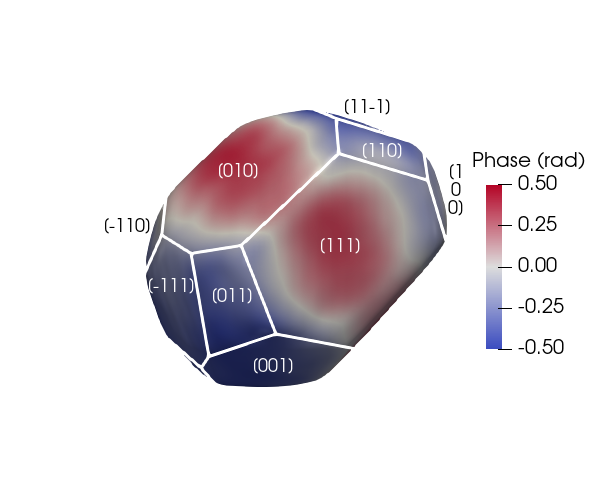
\includegraphics[trim=50 50 130 100, clip, width=\textwidth]{Figures/bcdi_data/D6/D6_facets.png}
            \label{fig:facets_D6}
        \end{figure}

        \column[T]{0.55\textwidth}
        \centering
        B: $\diameter \approx 350 nm$ 

        \begin{figure}
            \centering
            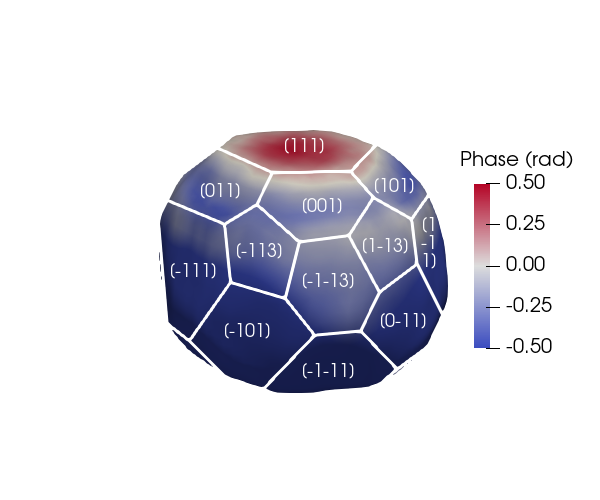
\includegraphics[trim=50 50 0 100, clip, width=\textwidth]{Figures/bcdi_data/B7/B7_facets.png}
            \label{fig:facets_B7}
        \end{figure}

    \end{columns}

    \pause
    \centering
    \vspace{-1em}
    \begin{itemize}
        \item \textcolor{Important}{Difference in size, shape, and in the type of facets exhibited.}
        \pause
        \item Most of the facets have low miller indices, (100), (110), (111).
        \pause
        \item The smaller nanoparticle has more 'open' facets such as Pt (311)
        \pause
        \item The area between different facets in considered to be edges or corners, depending on the coordination geometry.
    \end{itemize}
    
\end{frame}
    \begin{frame}{Strain field energy}

    \begin{columns}
        \column[T]{0.7\textwidth}

        \begin{figure}
            \centering
            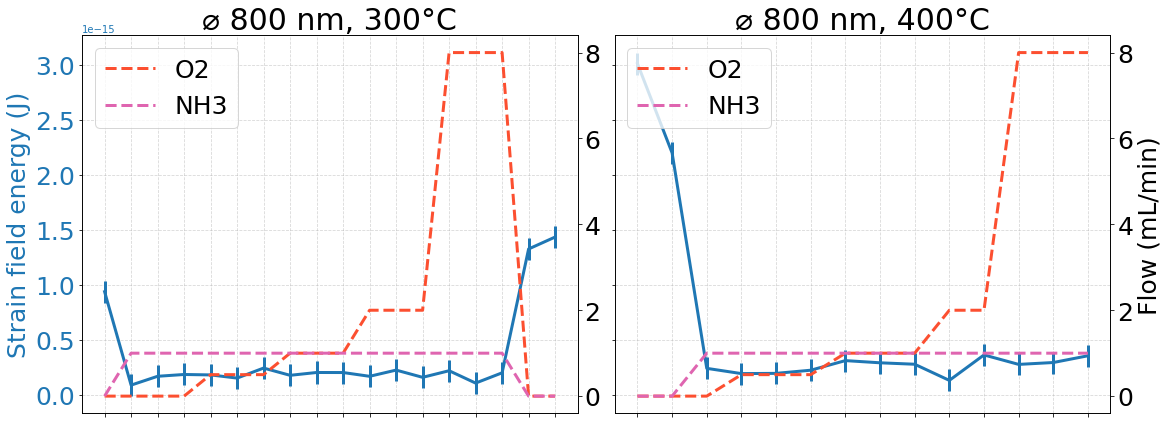
\includegraphics[width=\textwidth]{Figures/bcdi_data/D6/strain_energy_D-6.png}
            \onslide<2->{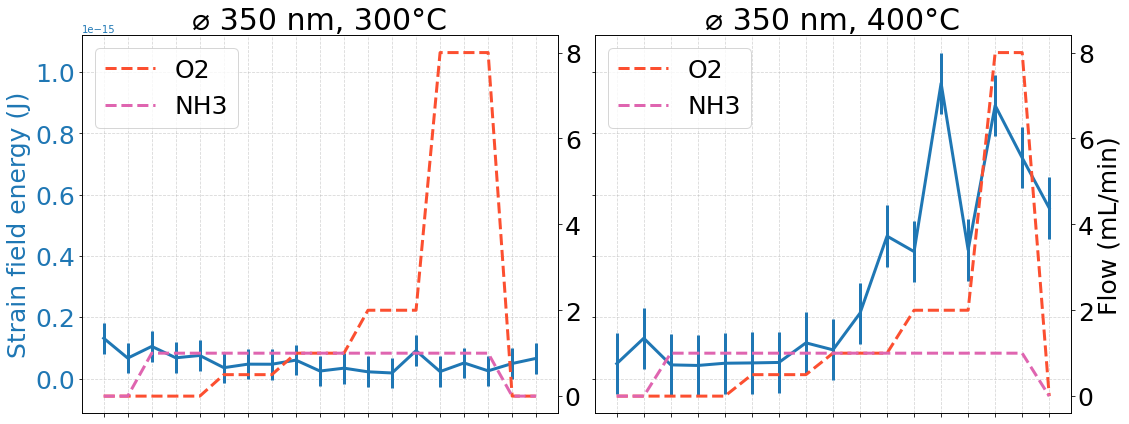
\includegraphics[width=0.51\textwidth, clip=True, trim=0 0 19.5cm 0]{Figures/bcdi_data/B7/strain_energy_B-7.png} }\hspace{-0.15cm}
            \onslide<3->{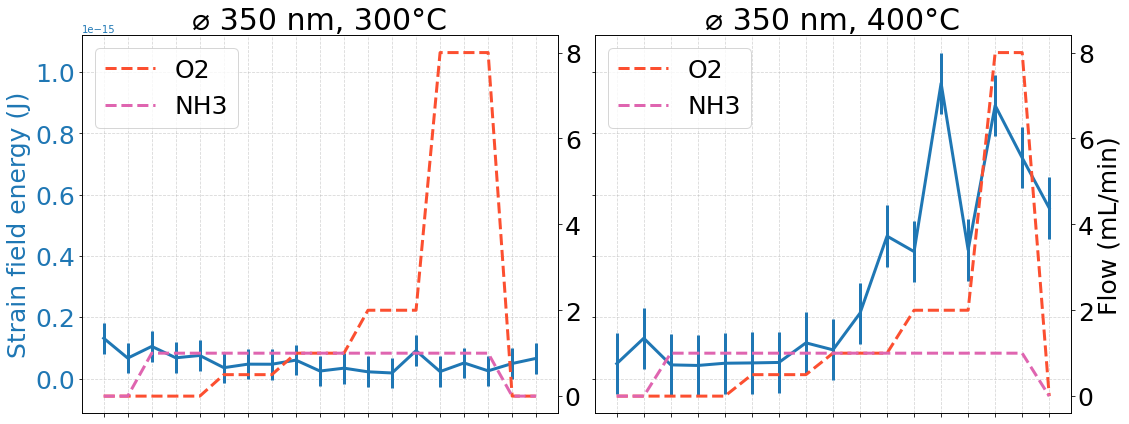
\includegraphics[width=0.48\textwidth, clip=True, trim=20.9cm 0 0 0]{Figures/bcdi_data/B7/strain_energy_B-7.png}}
            \caption{Strain field energy evolution with \ammonia and \dioxygen partial pressures.}
            \label{fig:SFE}
        \end{figure}

        \column[T]{0.3\textwidth}
        \begin{flushleft}
        \begin{equation*}
            E = \frac{A}{V} \int \Big( \frac{\partial u_{111}}{\partial x_{111}} \Big)^2dV %\frac{2G + 3I}{2}
        \end{equation*}
        \end{flushleft}

    \end{columns}
    
\end{frame}


\begin{frame}{Strain field energy}

    \begin{columns}
        \column[T]{0.7\textwidth}

        \begin{figure}
            \centering
            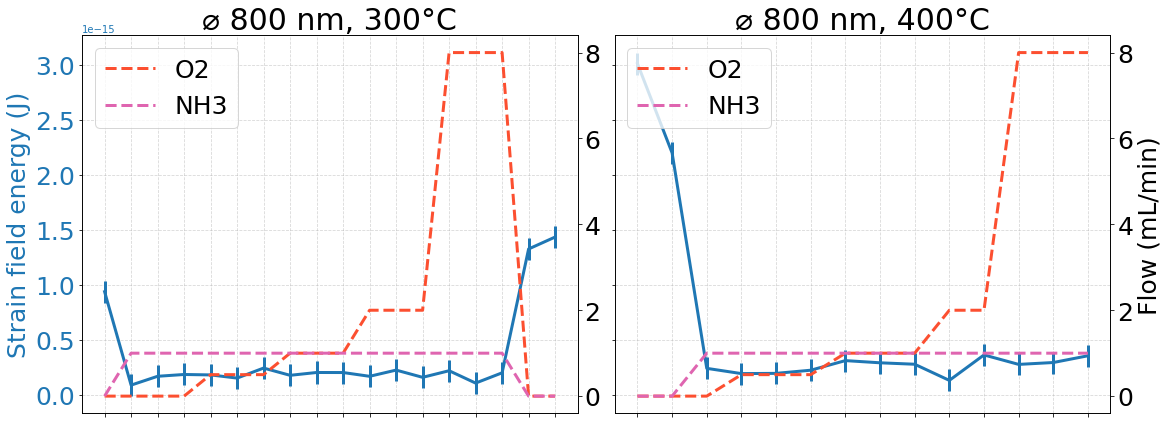
\includegraphics[width=\textwidth]{Figures/bcdi_data/D6/strain_energy_D-6.png}
            {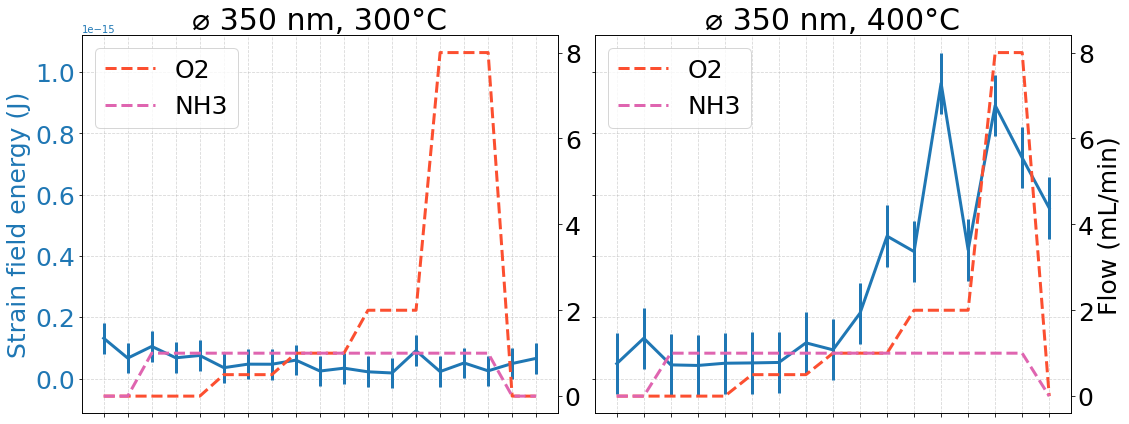
\includegraphics[width=0.51\textwidth, clip=True, trim=0 0 19.5cm 0]{Figures/bcdi_data/B7/strain_energy_B-7.png} }\hspace{-0.15cm}
            {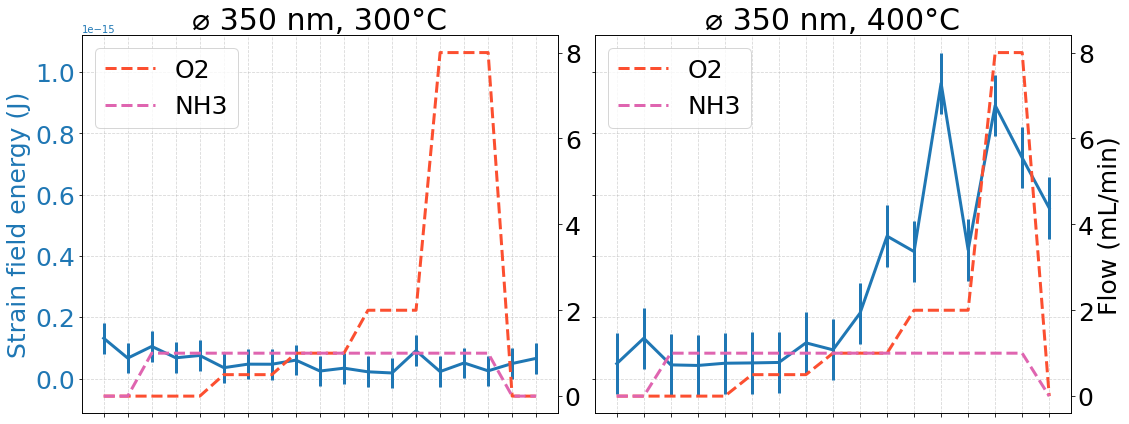
\includegraphics[width=0.48\textwidth, clip=True, trim=20.9cm 0 0 0]{Figures/bcdi_data/B7/strain_energy_B-7.png}}
            \caption{Strain field energy evolution with \ammonia and \dioxygen partial pressures.}
        \end{figure}

        \column[T]{0.3\textwidth}
        \begin{flushleft}
        \begin{equation*}
            E = \frac{A}{V} \int \Big( \frac{\partial u_{111}}{\partial x_{111}} \Big)^2dV %\frac{2G + 3I}{2}
        \end{equation*}
        \end{flushleft}
        
        \centering
        {\animategraphics[autoplay,loop, width=0.9\textwidth]{5}{Figures/bcdi_data/B7/MeshGif/3122_amp}{1}{20}}

    \end{columns}
    
\end{frame}


\begin{frame}{Strain field energy}

    \begin{columns}
        \column[T]{0.7\textwidth}

        \begin{figure}
            \centering
            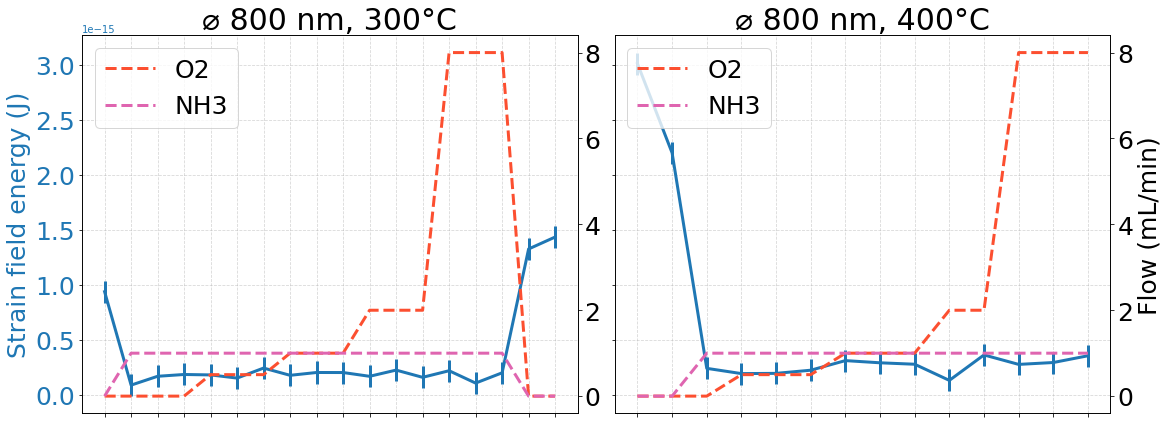
\includegraphics[width=\textwidth]{Figures/bcdi_data/D6/strain_energy_D-6.png}
            {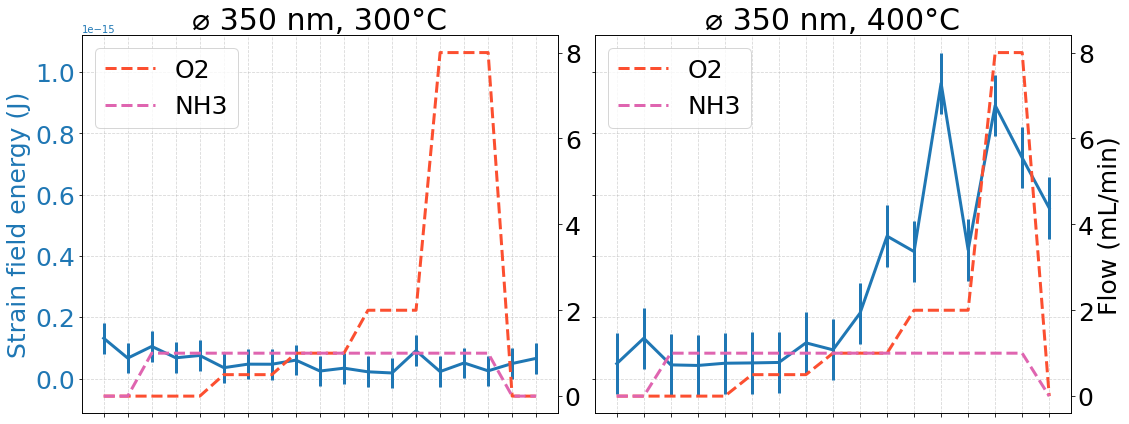
\includegraphics[width=0.51\textwidth, clip=True, trim=0 0 19.5cm 0]{Figures/bcdi_data/B7/strain_energy_B-7.png} }\hspace{-0.15cm}
            {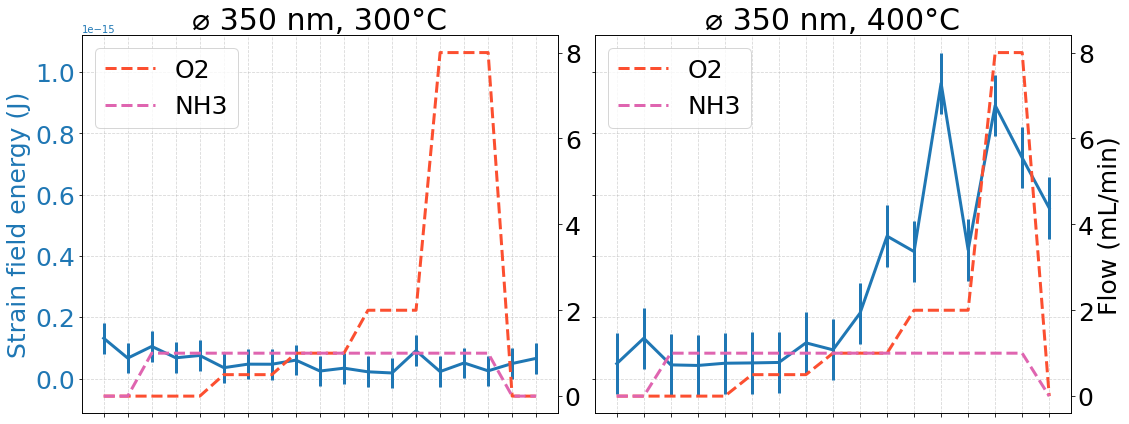
\includegraphics[width=0.48\textwidth, clip=True, trim=20.9cm 0 0 0]{Figures/bcdi_data/B7/strain_energy_B-7.png}}
            \caption{Strain field energy evolution with \ammonia and \dioxygen partial pressures.}
        \end{figure}

        \column[T]{0.3\textwidth}
        \begin{flushleft}
        \begin{equation*}
            E = \frac{A}{V} \int \Big( \frac{\partial u_{111}}{\partial x_{111}} \Big)^2dV %\frac{2G + 3I}{2}
        \end{equation*}
        \end{flushleft}
        
        \centering
        {\animategraphics[autoplay,loop, width=0.9\textwidth]{5}{Figures/bcdi_data/B7/MeshGif/3122_amp}{1}{20}}
        {\animategraphics[autoplay,loop, width=0.9\textwidth]{5}{Figures/bcdi_data/B7/MeshGif/4090_amp}{1}{20}}

    \end{columns}
    
\end{frame}

    \section{Surface X-ray Diffraction}
    % \begin{frame}{Six-circle diffractometer}

    \begin{columns}
    
        \column[T]{0.5\textwidth}
        \begin{itemize}
            \item $\beta_{in}$ is the incidence angle
            \item $\beta_{out}$ the outgoing angle
            \item $\gamma$ is the out-of-plane detector angle
            \item $\delta$ is the in-plane detector angle
            \item $\omega$ is the sample rotation around the axis perpendicular to the surface or sample azimuth.
        \end{itemize}
        
        In the z-axis mode, $h$ and $k$ are  the in-plane diffraction indices and $l$ is the out-of-plane diffraction index (often perpendicular to the surface). 
        
        $\vec{Q}$ is  the  momentum  transfer: 
        
        \begin{gather}
            \vec{Q} = \Vec{K_f} - \Vec{K_i} \\
            \vec{Q}_{par} = \vec{Q_x} + \vec{Q_y} \\
            \vec{Q_{perp}} = \vec{Q_z}
        \end{gather}
    
        \column[T]{0.5\textwidth}
        \centering
        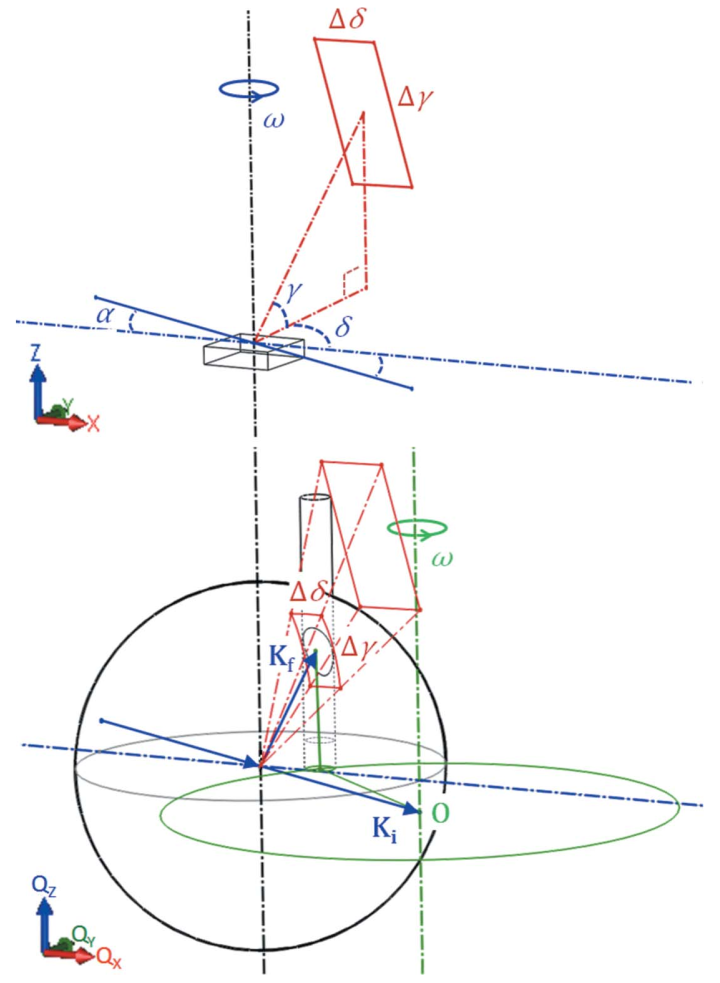
\includegraphics[width=0.8\textwidth]{Figures/sxrd_data/diffracto.png}
    
    \end{columns}

\end{frame}


\begin{frame}{Reciprocal space sampling}

    The integrated intensity of an ideal rocking ($\omega$) scan (i.e. intensity recorded while continuously rotating the sample around its surface normal) is:
    
    \begin{equation}
        I_\omega = \frac{\Phi_0}{\omega_0} \frac{A}{A_u} \int \int \int r_e^2 |F_{hkl}|^2 P u(Q) d\gamma d\delta d\omega
    \end{equation}
    
    \begin{itemize}
        \item $\Phi_0$ incident flux
        \item $\omega_0$ rotation speed
        \item $A$ active surface area
        \item $A_u$ area of the surface unit cell
        \item $|F_{hkl}$ structure factor of the reflection
        \item $P$ polarization factor
        \item and $u(Q)$ line shape function \footnotemark
    \end{itemize}
    
    Omega scans are discrete, with $T_\omega$ the acquisition time and $N_\omega$ points.
    
    \footnotetext{Drnec, J., Zhou, T., Pintea, S., Onderwaater, W., Vlieg, E. (2014). Integration techniques for surface X-ray diffraction data obtained with a two-dimensional detector. Journal of Applied Crystallography, 47, 365–377}

\end{frame}


\begin{frame}{Integrated intensity: rocking scan}

    As the Lorentz factor (L) and polarization factor (P) change with diffraction angle, corrections are necessary to obtain a correct profile, particularly for broad profiles.
    $I_\omega$ can be rewritten with the following correction factors \footnotemark:
    
    \begin{equation}
        I_\omega = \Phi_0 T_\omega \frac{A}{A_u^2} r_e^2 \lambda^2 |F_{hkl}|^2 P C_{area} C_{beam} C_{det} \frac{\Delta\gamma \cos \gamma}{\cos \alpha \sin \delta \cos \gamma}
    \end{equation}
    
    \begin{itemize}
        \item $C_{area}$ area correction factor, proportional to the illuminated surface area, defined by the size of the beam parallel to the surface and by the opening of the slits
        \item $C_{beam}$ compensates for the incoming beam intensity distribution profile
        \item $C_{det}$ present if the in-plane acceptance of the detector is not sufficiently large enough to cover the whole peak
        \item $\frac{1}{\cos \alpha \sin \delta \cos \gamma}$ is the Lorentz factor for the $\omega$ scan
        \item $\cos \gamma$ is the rod interception factor, integration correction dependent on the geometry of the rod–detector interception, assuming that $|F_{hkl}|$ is invariant along $l$ within the considered integration volume
    \end{itemize}
    
    \footnotetext{Vlieg, E. (1997).J. Appl. Cryst.30, 532–543}

\end{frame}

\begin{frame}{Integrated intensity: stationary measurement}

    In the case of a stationary scan, a single data acquisition of duration $T_s$ is carried out at a specific point in the reciprocal space.
    If we consider the in-plane detector acceptance to be larger than the cross section of the rod and $|F_{hkl}|$ to be invariant along $l$ within the intersected area, we have:
    
    \begin{equation}
        I_\omega = \Phi_0 T_\omega \frac{A}{A_u^2} r_e^2 \lambda^2 |F_{hkl}|^2 P C_{area} C_{beam} C_{det} \frac{1}{\sin \gamma}
    \end{equation}
    
    where $\frac{1}{\sin \gamma }$ is the Lorentz factor for the stationary measurements\footnotemark.
    
    \footnotetext{Vlieg, E. (1997).J. Appl. Cryst.30, 532–543}
\end{frame}


\begin{frame}{ROD integration}

    \begin{columns}
    
        \column[T]{0.5\textwidth}

        A complete rod intensity profile is measured through a series of rocking scans at different $l$ values. By using two-dimensional detectors, it is possible to replace each rocking scan by one single stationary measurement centered on the rod at the same $l$ value, speeding up data acquisition. However, certain conditions must be fulfilled:

        \begin{itemize}
            \item The in-plane projection of the finite acceptance of the detector expanded by $K_f\Delta\gamma\sin\gamma$ and $K_f\Delta\delta$ should be sufficiently large to fully include the cross section of the rod. This is not always true as $sin \gamma$ vanishes at $\gamma = 0$. Hence, for low $l$ values, one often has to employ a rocking scan or attempt to compensate for the missing intensity either analytically or numerically.
            \item $|F_{hkl}|$ should be approximately constant over the intersected $l$ range $\Delta l$.
        \end{itemize}
    
        \column[T]{0.5\textwidth}
        \centering
        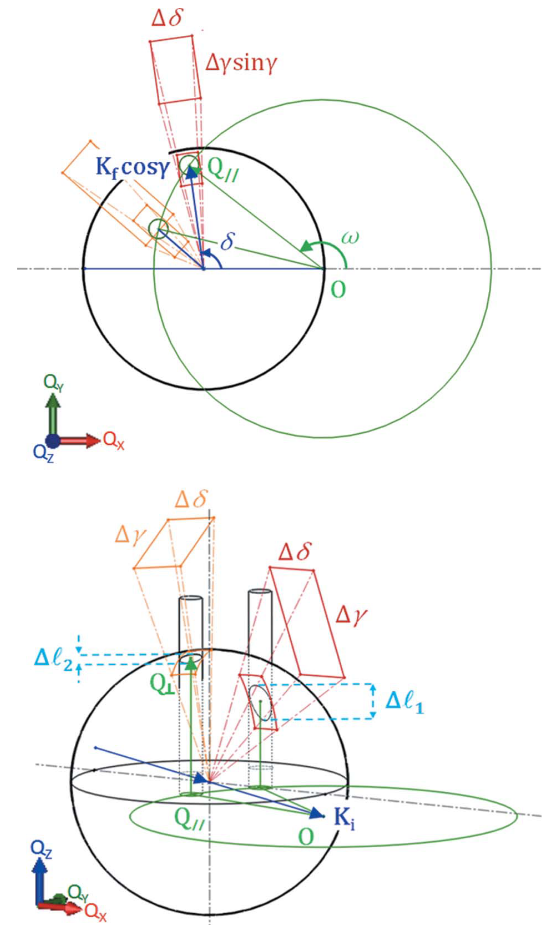
\includegraphics[width=0.7\textwidth]{Figures/sxrd_data/rod_integration.png}
    
    \end{columns}

\end{frame}


\begin{frame}{Background estimation}

    \begin{itemize}
        \item The field of view of the detector should be large enough to fully intersect the rod and accept an area with background intensity.
        \item Over (or under)-estimation of the background may result in significant errors.
        \begin{enumerate}
            \item Calculate the overall integrated intensity inside a region of interest (RoI) covering the intercepted rod
            \item Subtract the background intensity taken elsewhere.
        \end{enumerate}
        \item Signals coming from outside the sample may be found in close vicinity to the peak or even overlapping the peak, making it impossible to isolate the peak from the background with a regularly shaped RoI (e.g.rectangle).
        \item Applying an irregularly shaped RoI (e.g.a polygon) can solve the problem but requires the RoI to be determined for each image as the peak shape evolves during the scan.
        \item An alternative is to use peak shape determination and background subtraction employing a two-dimensional \textbf{peak search algorithm, detailed in Vlieg et al. (2016)}.
    \end{itemize}

    \centering
    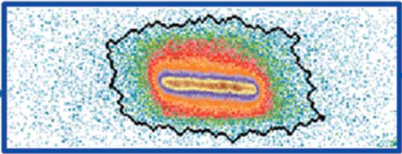
\includegraphics[height=0.25\textheight]{Figures/sxrd_data/SXRD_peak.png}
    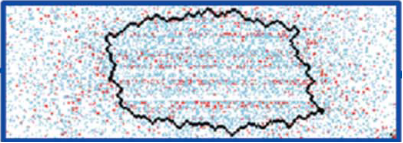
\includegraphics[height=0.25\textheight]{Figures/sxrd_data/SXRD_peak_background.png}
        
\end{frame}


\begin{frame}{Reciprocal space integration}

    The integrated intensity of a given volume in the angular space of the detector is:
    
    \begin{equation}
        I_{int,a} = \Phi_0 T_r \int \int \int \frac{d\sigma}{d\Omega}(\vec{Q})d\gamma d\psi d\phi
    \end{equation}
    
    where $\Phi_0$ is the incident flux, $T_r$ the counting time, $\frac{d\sigma}{d\Omega}(\vec{Q})$ the differential cross section and $d\gamma d\psi d\phi$ is the integration volume.
    
    The Lorentz correction, $L$, accounts for the angular to reciprocal space volume transformation:
    $d\gamma  d\psi d\phi = \frac{\lambda^3}{V_u} L \, dh \, dk \, dl$. In reciprocal space:
    
    \begin{gather}
        I_{int,r} = \Phi_0 T_r \int \int \int \frac{d\sigma}{d\Omega}(\vec{Q})\, dh \, dk \, dl \\
        I_{int,a} = \frac{\lambda^3}{V_u} L I_{int,r}
    \end{gather}
    
    where $V_u$ is the volume of the unit cell. For stationnary scans we have instead:
    
    \begin{equation}
        I_{int,a} = \frac{\lambda^2}{A_u} L I_{int,r}
    \end{equation}
    
    where $A_u$ is the area of the surface unit cell. The Lorentz correction is included when the pixel intensities of two-dimensional images are converted to the three-dimensional reciprocal space intensity map.

\end{frame}

\begin{frame}{Structure factor}

    The range in $l$ direction, $\Delta l$, measured by a detector is not constant and varies with the component of the scattering vector perpendicular to the surface ($\vec{Q_{perp}}$) and the angle $\gamma$ in the angular space of a detector.

    \begin{itemize}
        \item This is taken into account with the $\cos \gamma$ rod interception factor.
        \item If the integration is done directly in reciprocal space, $\Delta l$ can be chosen to be the same for each $l$ value given that the reciprocal space map has enough data points.
    \end{itemize}
    
    Assuming that $\Delta l$ is small enough so that $\frac{d\sigma}{d\Omega}(\vec{Q})$ is constant within $\Delta l$ we can write:

    \begin{align}
        I_{int,r} = \Phi_0 T_r \int \int \int \frac{d\sigma}{d\Omega}(\vec{Q})\, dh \, dk \, dl \\
        = \Phi_0 T_r \Delta l \int \int \frac{d\sigma}{d\Omega}(\vec{Q})\, dh \, dk \\
        = \Phi_0 T_r \frac{A}{A_u} r_e^2 |F_{hkl}|^2 P C_{area} C_{beam} \Delta l 
    \end{align}


    The $C_{det}$ correction is omitted because, it is possible to recover the in-plane shape and intensity distribution of the rod even if the post sample slit width is smaller than the width of the reflection at the camera distance.
        
\end{frame}

\begin{frame}{Rod integration}

    \begin{itemize}
        \item Is it correct to perform interpolations in the hk plane ?
        \item Do you have $\frac{\partial F_{hkl}}{\partial l} = 0$ ? Is it the correct step in l ?
        \item If in reciprocal space, have you well aligned the sample ? Does the peak move ?
        \item Have you correctly subtracted the background ? I.e. did you take care to see if there are alien peaks / background features ?
        \item Did you fit or integrate the CTR ? Recalculated  or integrated intensities ? Peak shape ?
    \end{itemize}

    \begin{figure}
        \centering
        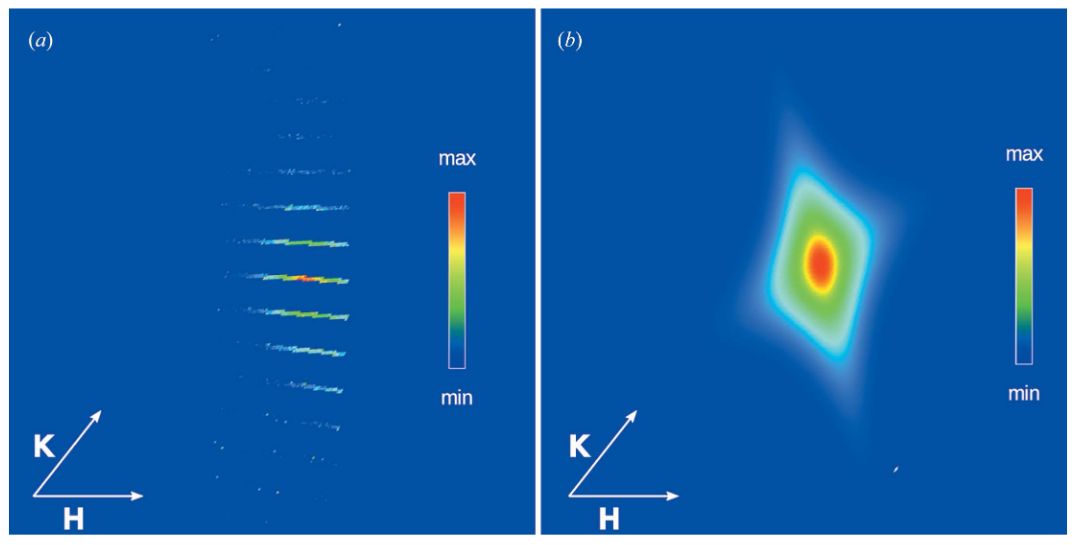
\includegraphics[width=0.6\textwidth]{Figures/sxrd_data/LorentzianFit.png}
        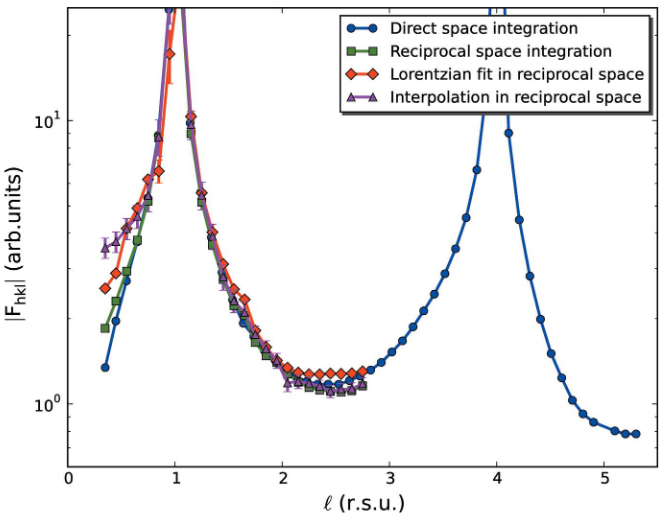
\includegraphics[width=0.38\textwidth]{Figures/sxrd_data/int_dif_sxrd.png}
        \caption{Lorentzian fit (left) and differences in data integration (right).}
        \label{fig:sxrd_data}
    \end{figure}
    
\end{frame}
    \begin{frame}{Surface X-ray diffraction}
    \begin{columns}
        \column[T]{0.35\textwidth}
        \centering
        \begin{itemize}
            \item SXRD allows us to probe the last layers of the crystal structure
            \vspace{0.25cm}
            \pause
            \item Study \textcolor{Important}{single facets} with the same setup and conditions, Pt (100), (111), ...
            % \pause
            % \item Expected results are surface reconstructions and the formation of new surface structures
            \vspace{0.25cm}
            \pause
            \item \textcolor{Important}{Explore correlation between specific facets and reaction products}
        \end{itemize}

        \centering
        \pause
        \begin{figure}
            \centering
            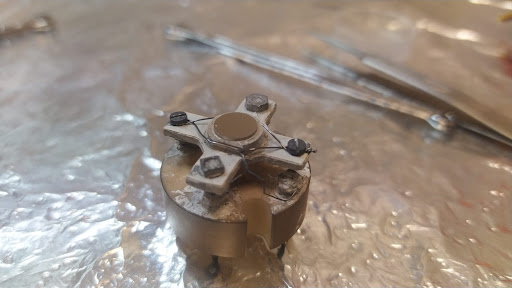
\includegraphics[width=0.9\textwidth, trim={3.5cm 3.5cm 5cm 3.5cm}, clip]{Figures/sxrd_data/sample_sxrd.jpg}
            \caption{Pt monocrystal used during Surface X-ray Diffraction.}
            \label{fig:my_label}
        \end{figure}

        % \pause
        % \begin{figure}
        %     \centering
        %     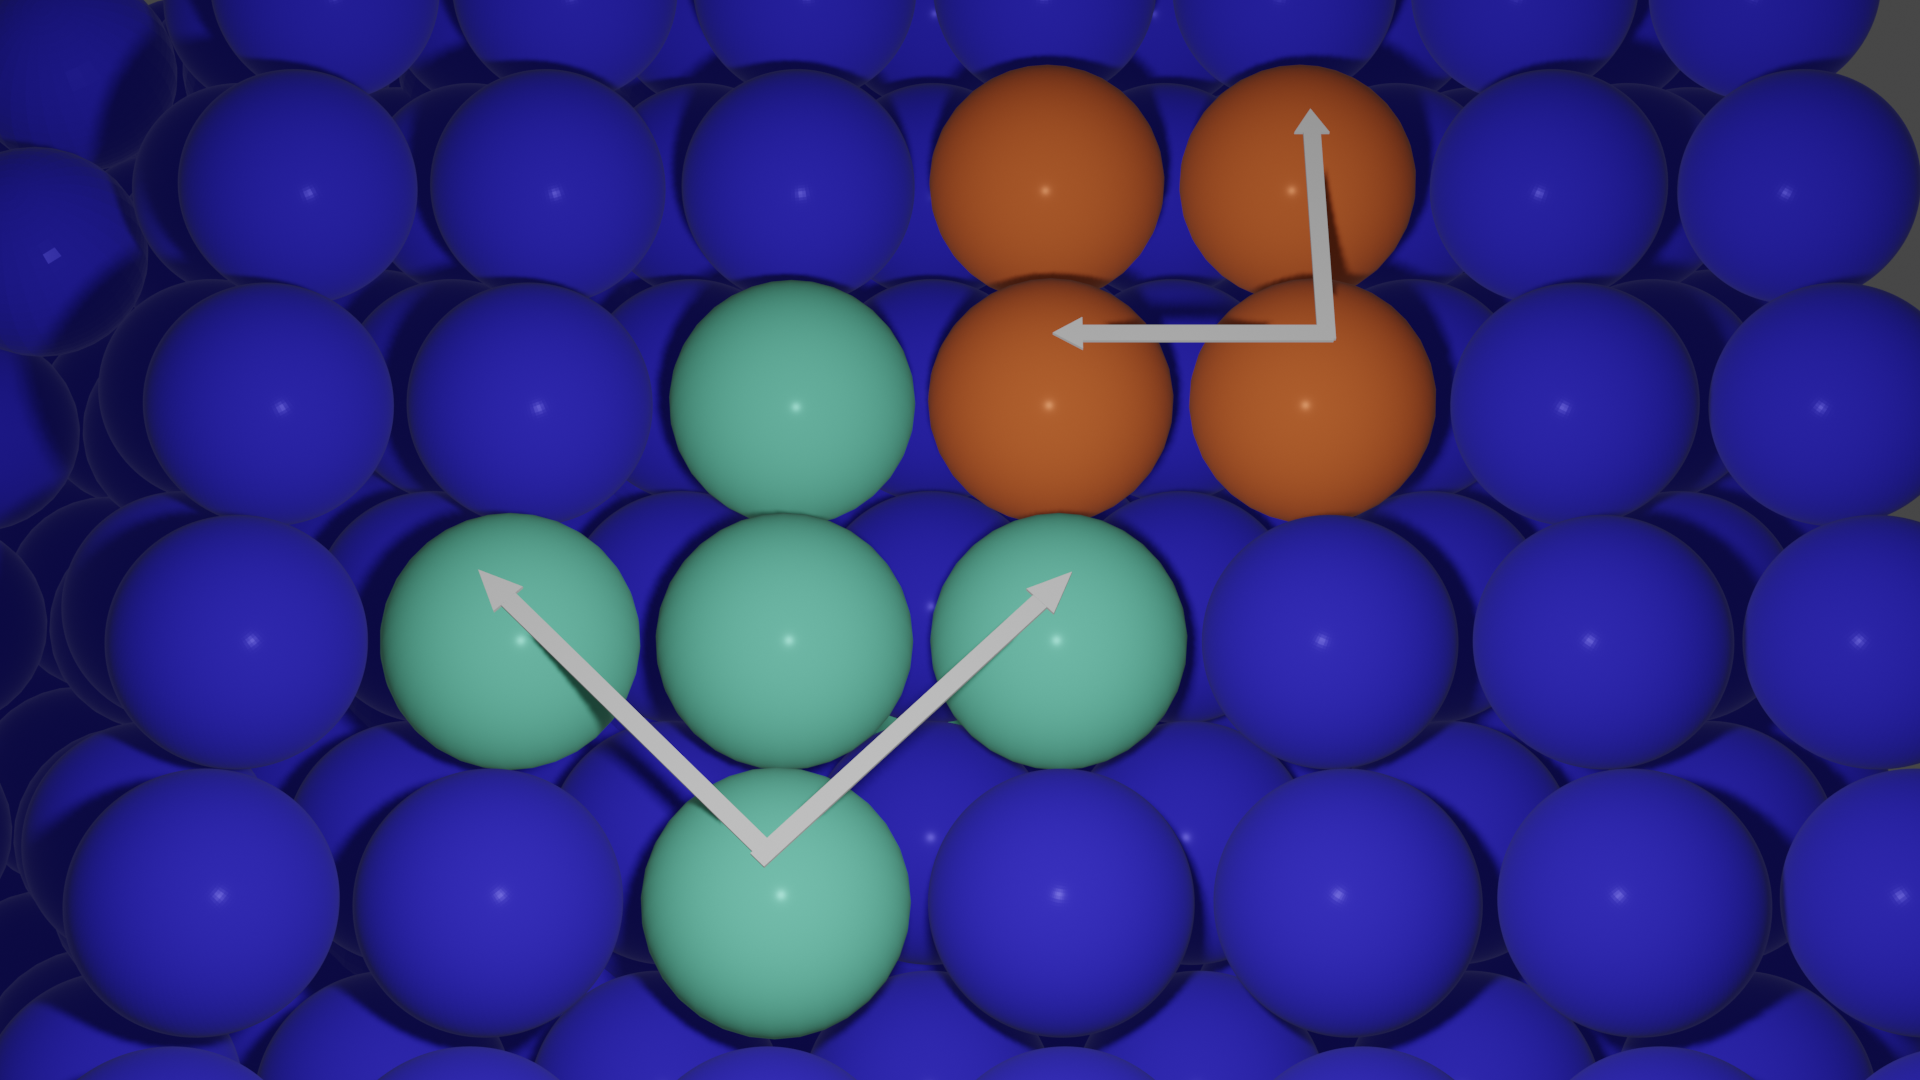
\includegraphics[width=0.8\textwidth]{Figures/sxrd_data/Pt100_blender.png}
        %     \caption{Pt (001) bulk unit cell (green) and surface unit cell (orange).}
        %     \label{fig:pt100_unit_cells}
        % \end{figure}

        \column[T]{0.65\textwidth}
        \pause
        \begin{figure}
            \centering
            \includegraphics[width=0.65\textwidth]{Figures/sxrd_data/PtOxides.png}
            \caption{Crystal  structure  of  platinum  oxides expected on Pt (100): (a) $PtO$; (b) \ptthreeofour;(c) $\alpha-PtO_2$; and (d) $\beta-PtO_2$ \footnotemark{}.\\ \textcolor{orange}{Platinum} and \textcolor{red}{Oxygen} atoms.}
            \label{fig:PtOstructures}
        \end{figure}

    \end{columns}
    
    \footnotetext{Seriani, N., Pompe, W., Ciacchi, L. (2006). Catalytic oxidation activity of Pt3O4 surfaces and thin films. Journal of Physical Chemistry B, 11(30), 14860–14869.}

\end{frame}
    % \begin{frame}{Possible structures}

Bulk Pt, FCC

Surface orientation

    $a=b=c=\SI{2.7748}{\angstrom}$\\
    $\alpha=\beta=\gamma=90°$

Bulk orientation

    $a=b=c = \SI{3.9242}{\angstrom}$\\
    $\alpha=\beta=\gamma=90°$

Hexagonal surface structure

    $a=b=c = \SI{3.32976}{\angstrom}$\\

    $\alpha=\beta=120°$
    $\gamma=90°$

\ptthreeofour, simple cubic, $a = \SI{5.48}{\angstrom}$
    
\end{frame}
    % \begin{frame}{Map at room temperature prior to the experiment}
    \begin{columns}
    
    \column[T]{0.35\textwidth}

    \column[T]{0.6\textwidth}
    
        \begin{figure}
        \centering
        \includegraphics[width=0.9\textwidth]{Figures/sxrd_data/maps/Map_hkl_surf_or_602-651.png}
        \caption{Pt [100] bulk-terminated structure reciprocal space map. RT}
        \label{fig:ArgonRT}
    \end{figure}
        
    \end{columns}

\end{frame}
    \begin{frame}{Ammonia oxidation cycle on Pt (100) at 400\degree C }
    \begin{columns}
    
    \column[T]{0.38\textwidth}
    \begin{table}
        \centering
        \begin{tabular}{ |l|l|l|l| }
            \hline
            Argon & \ammonia & \dioxygen & Duration \\
             & & & (hours) \\ 
            \hline
            \rowcolor{shadecolor}
            50 & 0 & 0 & 24 \\
            42 & 0 & 8 & 12 \\
            41 & 1 & 8 & 5 \\
            \hline
            50 & 0 & 0 & 7 \\
            42 & 0 & 8 & 1 \\
            41 & 1 & 8 & 10 \\
            48.5 & 1 & 0.5 & 13 \\
            49 & 1 & 0 & 11 \\
            50 & 0 & 0 & 8 \\
            \hline
        \end{tabular}
        \caption{Gas flow in reactor ($50$ mL/min, $0.3$ bar). In experimental order.}
    \end{table}

    Extinction conditions for Pt (FCC) are $h+k = 2n+1$ at $l=0$. 
    %Heating and sputter annealing under Argon removed the previous peaks.

    \column[T]{0.6\textwidth}
    
    \begin{figure}
        \centering
        \includegraphics[trim=0 0 40 0, clip, width=\textwidth]{Figures/sxrd_data/maps/Map_hkl_surf_or_1335-1375.png}
        \caption{Pt [100] bulk-terminated structure \\ reciprocal space in-plane map.}
        \label{fig:ArgonBefore}
    \end{figure}
        
    \end{columns}

\end{frame}
    \begin{frame}{Pt$_3$O$_4$ structure appears with oxygen}
    \begin{columns}
    
    \column[T]{0.35\textwidth}
    \begin{table}
        \centering
        \begin{tabular}{ |l|l|l|l| }
            \hline
            Argon & \ammonia & \dioxygen & Duration \\
             & & & (hours) \\ 
            \hline
            50 & 0 & 0 & 24 \\
            \rowcolor{shadecolor}
            42 & 0 & 8 & 12 \\
            41 & 1 & 8 & 5 \\
            % \hline
            % 50 & 0 & 0 & 7 \\
            % 42 & 0 & 8 & 1 \\
            % 41 & 1 & 8 & 10 \\
            % 48.5 & 1 & 0.5 & 13 \\
            % 49 & 1 & 0 & 11 \\
            % 50 & 0 & 0 & 8 \\
            \hline
        \end{tabular}
        \caption{Gas flow in reactor ($50$ mL/min, $0.3$ bar). In experimental order.}
    \end{table}

    \vspace{-0.5cm}

    \begin{figure}
        \centering
        \includegraphics[width=\textwidth]{Figures/sxrd_data/ctr/reconstruction_ctr_pt3o4.png}
        % \includegraphics[width=\textwidth]{Figures/sxrd_data/ctr/reconstruction_ctr_pt3o4_no_data.png}
        \caption{CTR, peaks at L={0.7, 1.4, 2.1, 2.8} are characteristic of Pt$_3$O$_4$.}
        \label{fig:ctr_pt3o4}
    \end{figure}
    
    \column[T]{0.6\textwidth}
    
        \begin{figure}
            \centering
            \includegraphics[width=0.9\textwidth]{Figures/sxrd_data/maps/Map_hkl_surf_or_1596-1635.png}
            \caption{Reciprocal space in-plane map with high oxygen atmosphere. The presence of oxygen induces two surface structures, \ptthreeofour and a yet \textcolor{green}{unknown structure} that is slightly shifted (no structure in L). }
            \label{fig:CondF1}
        \end{figure}
    
    \end{columns}

\end{frame}
    \begin{frame}{Adding Ammonia}
    \begin{columns}
    
    \column[T]{0.38\textwidth}
    \begin{table}
        \centering
        \begin{tabular}{ |l|l|l|l| }
            \hline
            Argon & \ammonia & \dioxygen & Duration \\
             & & & (hours) \\ 
            \hline
            50 & 0 & 0 & 24 \\
            42 & 0 & 8 & 12 \\
            \rowcolor{shadecolor}
            41 & 1 & 8 & 5 \\
            \hline
            50 & 0 & 0 & 7 \\
            42 & 0 & 8 & 1 \\
            41 & 1 & 8 & 10 \\
            48.5 & 1 & 0.5 & 13 \\
            49 & 1 & 0 & 11 \\
            50 & 0 & 0 & 8 \\
            \hline
        \end{tabular}
        \caption{Gas flow in reactor ($50$ mL/min, $0.3$ bar). In experimental order.}
    \end{table}

    The addition of Ammonia removes the second structure, but the peaks linked to \ptthreeofour are still here.

    \column[T]{0.6\textwidth}
    
    \begin{figure} % pb here
        \centering
        \includegraphics[trim=0 0 40 0, clip, width=0.95\textwidth]{Figures/sxrd_data/maps/Map_hkl_surf_or_1880-1902.png}
        \caption{Reciprocal space in-plane map under reacting conditions. The heater broke during this map and the temperature difference resulted in a loss of alignment.}
        \label{fig:CondE1}
    \end{figure}
        
    \end{columns}

\end{frame}
    \begin{frame}{Transient structure during deactivation}
    \begin{columns}
    
    \column[T]{0.38\textwidth}
    \begin{table}
        \centering
        \begin{tabular}{ |l|l|l|l| }
            \hline
            Argon & \ammonia & \dioxygen & Duration \\
             & & & (hours) \\ 
            \hline
            50 & 0 & 0 & 24 \\
            42 & 0 & 8 & 12 \\
            41 & 1 & 8 & 5 \\
            \hline
            50 & 0 & 0 & 7 \\
            \rowcolor{shadecolor}
            42 & 0 & 8 & 1 \\
            41 & 1 & 8 & 10 \\
            48.5 & 1 & 0.5 & 13 \\
            49 & 1 & 0 & 11 \\
            50 & 0 & 0 & 8 \\
            \hline
        \end{tabular}
        \caption{Gas flow in reactor ($50$ mL/min, $0.3$ bar). In experimental order.}
    \end{table}

    Under high oxygen atmosphere, the same peaks reappear, characteristic of the two surface structures.

    \column[T]{0.6\textwidth}
    
        \begin{figure}
        \centering
        \includegraphics[trim=0 0 40 0, clip, width=0.95\textwidth]{Figures/sxrd_data/maps/Map_hkl_surf_or_1930-1936.png}
        \caption{Small reciprocal space in-plane map. After changing the heater, the sample was cleaned with two sputter annealing cycles (Ar).}
        \label{fig:CondF2}
    \end{figure}
        
    \end{columns}

\end{frame}
    \begin{frame}{\ptthreeofour surface reconstructions}
    \begin{columns}
    
    \column[T]{0.38\textwidth}

    \begin{overprint}
        \onslide<1>\begin{table}
        % \begin{table}
            \centering
            \begin{tabular}{ |l|l|l|l| }
                \hline
                Argon & \ammonia & \dioxygen & Duration \\
                 & & & (hours) \\ 
                \hline
                50 & 0 & 0 & 24 \\
                42 & 0 & 8 & \cellcolor{Important} 12 \\
                41 & 1 & 8 & 5 \\
                \hline
                50 & 0 & 0 & 7 \\
                42 & 0 & 8 & \cellcolor{Important} 1 \\
                \rowcolor{shadecolor}
                41 & 1 & 8 & 10 \\
                48.5 & 1 & 0.5 & 13 \\
                49 & 1 & 0 & 11 \\
                50 & 0 & 0 & 8 \\
                \hline
            \end{tabular}
            \caption{Gas flow in reactor ($50$ mL/min, $0.3$ bar). In experimental order.}
        \end{table}
        \onslide<2>\begin{figure}
            \centering
            \includegraphics[width=0.95\textwidth]{Figures/sxrd_data/ctr/reconstruction_ctr_condE.png}
            \caption{CTR, peaks at L={0.7, 1.4, 2.1, 2.8} are characteristic of \ptthreeofour (red dots). The background shape is linked to xxx. The peaks for the green dots are linked to xxx.}
            \label{fig:ctr_conde}
        \end{figure}
    \end{overprint}

    % add fit with ROD

    %\vspace{-0.5cm}

    The second structure does not disappear this time when adding \ammonia. Instead we have $10\times10$ reconstructions for \ptthreeofour.

    \column[T]{0.6\textwidth}

    \begin{figure}
        \centering
        \includegraphics[width=0.79\textwidth]{Figures/sxrd_data/maps/band_in_k_reconstructions.png}
        \caption{Reciprocal space in-plane map under reacting conditions (top) and map integration highlighting reconstruction peaks (bottom).}
        \label{fig:CondE2}
    \end{figure}
    \end{columns}
    
\end{frame}
    \begin{frame}{Surface hexagonal structure appearance}
    \begin{columns}
    
    \column[T]{0.38\textwidth}

    \begin{overprint}
        \onslide<1>\begin{table}
            \centering
            \begin{tabular}{ |l|l|l|l| }
                \hline
                Argon & \ammonia & \dioxygen & Duration \\
                 & & & (hours) \\ 
                \hline
                50 & 0 & 0 & 24 \\
                42 & 0 & 8 & 12 \\
                41 & 1 & 8 & 5 \\
                \hline
                50 & 0 & 0 & 7 \\
                42 & 0 & 8 & 1 \\
                41 & 1 & 8 & 10 \\
                \rowcolor{shadecolor}
                48.5 & 1 & 0.5 & 13 \\
                49 & 1 & 0 & 11 \\
                50 & 0 & 0 & 8 \\
                \hline
            \end{tabular}
            \caption{Gas flow in reactor ($50$ mL/min, $0.3$ bar). In experimental order.}
        \end{table}
        \onslide<2>\begin{figure}
            \centering
            \includegraphics[width=\textwidth]{Figures/sxrd_data/ctr/reconstruction_ctr_condB.png}
            \caption{CTR on white diamond primary reflections. No structure in L can be easily identified, but rather a continuous decrease of the signal,  characteristic of an unordered structure in $\Vec{c}$.}
            \label{fig:ctr_conde}
        \end{figure}
    \end{overprint}

    Not hexagonal $\alpha-$Pt$O_2$ ($|\Vec{a}| \approx \SI{3.10}{\angstrom}$). Matches with (111) of \ptthreeofour.
    
    \column[T]{0.6\textwidth}
    
    \begin{figure}
        \centering
        % \includegraphics[width=0.85\textwidth, trim={14cm 0 3.5cm 0}, clip]{Figures/sxrd_data/maps/Map_hkl_surf_or_hex_2227-2283.png}

        \includegraphics[trim=40 0 40 0, clip, width=0.9\textwidth]{Figures/sxrd_data/maps/Map_hkl_surf_or_2227-2283.png}
        \caption{Reciprocal space map. Atmospheres with low oxygen to ammonia ratio favour a hexagonal surface structure on Pt (100). Primitive cell (red or white diamond) $a=4.624, \gamma=120\degree$.}

        \label{fig:CondB}
    \end{figure}
    
    \end{columns}

\end{frame}
    \begin{frame}{Transient structure during deactivation}
    \begin{columns}
    
    \column[T]{0.38\textwidth}
    \begin{table}
        \centering
        \begin{tabular}{ |l|l|l|l| }
            \hline
            Argon & \ammonia & \dioxygen & Duration \\
             & & & (hours) \\ 
            \hline
            50 & 0 & 0 & 24 \\
            42 & 0 & 8 & 12 \\
            41 & 1 & 8 & 5 \\
            \hline
            50 & 0 & 0 & 7 \\
            42 & 0 & 8 & 1 \\
            41 & 1 & 8 & 10 \\
            48.5 & 1 & 0.5 & 13 \\
            \rowcolor{shadecolor}
            49 & 1 & 0 & 11 \\
            50 & 0 & 0 & 8 \\
            \hline
        \end{tabular}
        \caption{Gas flow in reactor ($50$ mL/min, $0.3$ bar). In experimental order.}
    \end{table}

    The intensity of the hexagonal structure decreases. It disappears without oxygen in the reactor.

    \column[T]{0.6\textwidth}
    
        \begin{figure}
        \centering
        \includegraphics[trim=0 0 40 0, clip, width=\textwidth]{Figures/sxrd_data/maps/Map_hkl_surf_or_2520-2570.png}
        \caption{Reciprocal space map with the same intensity scale as before.}
        \label{fig:CondA}
    \end{figure}
        
    \end{columns}

\end{frame}
    \begin{frame}{End the oxidation cycle with a clean surface}
    \begin{columns}
    
    \column[T]{0.38\textwidth}
    \begin{table}
        \centering
        \begin{tabular}{ |l|l|l|l| }
            \hline
            Argon & \ammonia & \dioxygen & Duration \\
             & & & (hours) \\ 
            \hline
            50 & 0 & 0 & 24 \\
            42 & 0 & 8 & 12 \\
            41 & 1 & 8 & 5 \\
            \hline
            50 & 0 & 0 & 7 \\
            42 & 0 & 8 & 1 \\
            41 & 1 & 8 & 10 \\
            48.5 & 1 & 0.5 & 13 \\
            49 & 1 & 0 & 11 \\
            \rowcolor{shadecolor}
            50 & 0 & 0 & 8 \\
            \hline
        \end{tabular}
        \caption{Gas flow in reactor ($50$ mL/min, $0.3$ bar). In experimental order.}
    \end{table}

    Removing the reagents brings back the Pt (100) bulk-terminated structure. \textcolor{Important}{The cycle is reproducible.}

    \column[T]{0.6\textwidth}
    
        \begin{figure}
        \centering
        \includegraphics[trim=40 0 40 0, clip, width=0.95\textwidth]{Figures/sxrd_data/maps/Map_hkl_surf_or_2719-2767.png}
        \caption{Pt (100) bulk-terminated structure reciprocal space map.}
        \label{fig:ArgonAfter}
    \end{figure}
        
    \end{columns}

\end{frame}

    \section{Conclusion}
    % \begin{frame}{References}
    \printbibliography

\end{frame}
    \begin{frame}{Conclusion}

    \begin{columns}
        \column[T]{0.38\textwidth}
        \vspace{1cm}
        \begin{itemize}
            \item Successfully measured Pt nanoparticles, providing insights into the size, shape and facet dependence.
            \pause
            \vspace{0.4cm}
            \item Different surface structures depending on reaction conditions on Pt (100)
            % \pause
            % \item Difference in the N 1s edge XPS spectra between Pt [100] and Pt [111] shows a difference in surface moieties.
            \pause
            \vspace{0.4cm}
            \item Continue analysis and  link the structural evolution with the catalytic activity.
        \end{itemize}

        \column[T]{0.58\textwidth}

        \pause
        \begin{figure}
            \centering
            \includegraphics[width=\textwidth]{Figures/sixs/MED.jpg}
        \end{figure}

        \vspace{0.5cm}
        \textit{We would like to thank all the SOLEIL, ESRF and CEA staff for the support and the ERC Carine that supported the research.}

    \end{columns}
\end{frame}

    % \begin{frame}{Scientific output and training}
    \begin{columns}
        \column[T]{0.58\textwidth}

        \textcolor{Prune}{Papers}
        \begin{itemize}
            \item Gwaihir (2022, JSR)
            \item Future : Ammonia oxidation, 3D BCDI
        \end{itemize}

        \pause
        \textcolor{Prune}{Conferences}
        \begin{itemize}
            \item AFC (poster) GDR CohereX (talk), Shanghai coherence (talk), SOLEIL user meeting (talk), EDPIF day (poster), ESRF UM 2022 (tutorial)
            \item Future: ESRF UM 2023 (tutorial), TMS San Diego (talk)
        \end{itemize}

        \pause
        \textcolor{Prune}{Courses}
        \begin{itemize}
            \item HERCULES, GDR Nanoperando, CDF, MOOC MPI, MOOC Intégrité, Sécurité Gaz, Machine Learning
            \item Future:  GDR CohereX 2023 ?
        \end{itemize}
        
        \pause
        \textcolor{Prune}{Teaching}
        \begin{itemize}
            \item TP 2022 (44h)
            \item TD 2023 (14h), TP 2023 (30h)
        \end{itemize}

        \column[T]{0.38\textwidth}
        
        \pause
        \textcolor{Important}{Last year of Phd goals}
        \begin{itemize}
            \item Finish analysis on Ammonia oxidation
            \item Start thesis writing in June ?
            \item Conference on SXRD ?
        \end{itemize}

        \vspace{1cm}

        \pause
        \textcolor{Prune}{Future}
        \begin{enumerate}
            \item Post-doc with a fully scientific project $+$ teaching $\rightarrow$ Maître de conférence
            \begin{itemize}
                \item Outside Europe ? $\rightarrow$ USA
                \item Grenoble (ESRF) ?
            \end{itemize}
            \item Post doc with code development: ESRF (VFN), SOLEIL ?
            \item Start-up or green industry (possible to join after code-oriented post-doc)
        \end{enumerate}
    \end{columns}
    
\end{frame}
    {\setbeamercolor{background canvas}{bg=DarkBlue}
\begin{frame}

    \centering

    \vspace{0.5cm}

    \includegraphics[height=1.2cm]{Figures/logo/logosixs.jpg} \hspace{1cm}
    \colorbox{white}{\includegraphics[height=1.2cm]{Figures/logo/SOLEIL.png}} \hspace{1cm}
    \includegraphics[height=1.2cm]{Figures/logo/CEA.png} \hspace{1cm}
    \includegraphics[height=1.2cm]{Figures/logo/ParisSaclayPrune.jpg}\\
    
    \vspace{2cm}

    \Large{\textcolor{white}{Thank you for listening !}}\\
    \vspace{1cm}
    \small{\textcolor{white}{david.simonne@synchrotron-soleil.fr}}\\
    
    \vspace{2cm}

    \includegraphics[height=1.2cm]{Figures/logo/logo_erc.png}\hspace{1cm}
    \includegraphics[height=1.2cm]{Figures/logo/logo_technion.png}\hspace{1cm}
    \colorbox{white}{\includegraphics[height=1.2cm]{Figures/logo/logocarine.png}}
    
\end{frame}
}

    %%%%%%%%%%%%%% APPENDIX %%%%%%%%%%%%%%%%
\appendix
    \begin{frame}{The material and pressure gap}

    \begin{columns}

        \column[T]{0.35\textwidth}
        
        \huge\textcolor{Important}{"A long standing conundrum in the catalysis community emerged at the interface between surface science and heterogeneous catalysis, better known as the pressure and materials gap."}
        
        \large\textcolor{Important}{Nature Catalysis editorial, 2018.}
        
        \column[T]{0.6\textwidth}

        Pressure gap:
        \begin{itemize}
            \item Typical industrial pressures between 1-12 bar and temperatures ranging from 1073-1223 K
            \item Most of the studies are performed at low pressures ($< 10^{-2} mbar$)
            \item Near-ambient pressure experiment
        \end{itemize}

        \vspace{2cm}
        Material gap:
        \begin{itemize}
            \item Platinum–rhodium wires, diameters in the range of 60–80 $\mu m$
            \item Pt nanoparticles and single crystals
        \end{itemize}

% Nowa- days, stacks of up to 50 knitted gauzes composed of platinum–rhodium wires with rhodium contents of 5–10 wt.% and wire diameters in the range of 60–80 μm have replaced the long term industry standard of woven platinum gauzes [2–4].

%cIn operation the catalyst gauzes undergo onsiderable reconstruction starting with smooth wires and ending with corroded wires covered with fractal structures in the shape of cauliflowers

    \end{columns}

\end{frame}
    
    \begin{frame}{Software architecture}

    \tikzstyle{mainblock} = [rectangle, rounded corners, minimum width=3cm, minimum height=2cm,text centered, draw=black, fill=red!30]
    \tikzstyle{arrow} = [thick,->,>=stealth]
    \vspace{0.2cm}
    \centering
    \begin{tikzpicture}[node distance=4cm]
        \node (controller) [mainblock, align=center] {Controller\\Workflow for fast analysis (pynx, bcdi, ...)};
        \node (result) [mainblock, right of=controller, yshift=-5cm, align=center] {Result\\Dataset class based on NeXuS architecture};
        %\node (logo) [right of=controller, xshift=2cm, yshift=1cm] {\includegraphics[width=.1\textwidth]{Figures/logo/pythonlogo.png}};
        
        \node (view) [mainblock, left of=controller, yshift=-5cm, align=center] {View\\Remote access GUI};
        
        \draw [arrow] (controller) |- node[anchor=north] {initializes} (view);
        \draw [arrow] [above] (view) |- node[anchor=south] {updates} (controller);
        \draw [arrow] [right] (controller) -| node[anchor=south] {overwrites} (result);
    \end{tikzpicture}
    
\end{frame}
    \begin{frame}{Software architecture}

    \tikzstyle{mainblock} = [rectangle, rounded corners, minimum width=3cm, minimum height=2cm,text centered, draw=black, fill=red!30]
    \tikzstyle{arrow} = [thick,->,>=stealth]
    \vspace{0.2cm}
    \centering
    \begin{tikzpicture}[node distance=4cm]
        \node (controller) [mainblock, align=center] {Controller\\Workflow for fast analysis (pynx, bcdi, ...)};
        \node (result) [mainblock, right of=controller, yshift=-5cm, align=center] {Result\\Dataset class based on\\NeXuS architecture};
        %\node (logo) [right of=controller, xshift=2cm, yshift=1cm] {\includegraphics[width=0.1\textwidth]{Figures/logo/pythonlogo.png}};
        
        \node (pgm) [left of=controller, xshift=0cm, yshift=-3cm] {\includegraphics[width=0.4\textwidth]{Figures/gwaihir/hackerman.png}};
        \node (text) [left of=controller, xshift=0cm, yshift=-5cm, align=center] {Advanced users can use terminal scripts \\
        for quick analysis.};

        \draw [arrow] [right] (controller) -| node[anchor=south] {overwrites} (result);
    \end{tikzpicture}
    
\end{frame}

    \begin{frame}{Facets retrieval}
    \begin{columns}
        \column[T]{0.48\textwidth}
        \begin{figure}
            \centering
            \includegraphics[width=\textwidth]{Figures/bcdi_data/facets_probability.png}
            \caption{A mesh is constructed from the particle voxels }
            \label{fig:particle_mesh}
        \end{figure}

        \column[T]{0.48\textwidth}

        A mesh of the surface is created by the marching-cubes algorithm, resulting in a surface made out of triangles, that in 3D can take up to 26 different orientations. 
        
        The surface is then smoothed to remove the steps created by the voxel size. 

        The main parameters to retrieve the facets are:
        \begin{itemize}
            \item facet normal direction
            \item facet size
            \item roughness tolerance
        \end{itemize}

        The entire procedure has been detailed in literature \footnotemark{}, but could benefit from a Python implementation.

        % Marching square :https://www.sciencedirect.com/topics/computer-science/marching-cube-algorithm
        %These define the tolerance for the roughness of ideally planar facets. 
        %Apart from the determination of the interplanar angles, the relative and absolute facet sizes, the facet normals and centers the main output also labels the faceted regions.
        %The second output of the plugin is an idealized hull of the input, constructed only from the facets found. 
        %The third output consists of the edges of this hull. 
        %Values that belong to two adjacent facets are assigned to these edges, like for example their interplanar angle.
        %The Sample Size, the Angle Uncertainty and the Splat Radius allow to tune the roughness tolerance

        % The Minimum Relative Facet Size allow to reduce the amount of the finally detected facets.

    \end{columns}

    
    \footnotetext{Facet Analyser: ParaView plugin for automated facet detection and measurement of interplanar angles of tomographic objects. Grothausmann, R., Beare, R. (2015) The MIDAS Journal}
\end{frame}
    \begin{frame}{Operando BCDI}

    \begin{figure}
        \centering
        \includegraphics[width=\textwidth]{Figures/bcdi_data/OperandoBCDI.png}
        %\caption{Caption}
        \label{fig:operando_bcdi}
    \end{figure}
    
\end{frame}

    \begin{frame}{Low oxygen pressure}
    \begin{columns}
    
    \column[T]{0.38\textwidth}
    \begin{table}
        \centering
        \begin{tabular}{ |l|l|l|l| }
            \hline
            Argon & \ammonia & \dioxygen & Duration \\
             & & & (hours) \\ 
            \hline
            50 & 0 & 0 & 24 \\
            42 & 0 & 8 & 12 \\
            41 & 1 & 8 & 5 \\
            \hline
            50 & 0 & 0 & 7 \\
            42 & 0 & 8 & 1 \\
            41 & 1 & 8 & 10 \\
            48.5 & 1 & 0.5 & 13 \\
            49 & 1 & 0 & 11 \\
            50 & 0 & 0 & 8 \\
            \hline
            50 & 0 & 0 & 8 \\
            \rowcolor{shadecolor}
            49.5 & 0 & 0.5 & 4 \\
            \hline
        \end{tabular}
        \caption{Gas flow in reactor ($50$ mL/min, $0.3$ bar). In experimental order.}
    \end{table}

    Multiple new peaks appear with only a \textcolor{Important}{very low amount of oxygen} in the reactor.

    \column[T]{0.6\textwidth}
    
        \begin{figure}
        \centering
        \includegraphics[trim=40 0 40 0, clip, width=\textwidth]{Figures/sxrd_data/maps/Map_hkl_surf_or_2905-2953.png}
        \caption{Reciprocal space map. The sample was cleaned with two sputter annealing cycles (Ar).}
        \label{fig:CondG}
    \end{figure}
        
    \end{columns}

\end{frame}
    \begin{frame}{Crystal truncation rods}
    \begin{columns}
        
    \column[T]{0.38\textwidth}
    \small{
    \begin{table}
        \centering
        \begin{tabular}{ |l|l|l|l| }
            \hline
            Argon & \ammonia & \dioxygen & Duration \\
             & & & (hours) \\ 
            \hline
            50 & 0 & 0 & 24 \\
            42 & 0 & 8 & 12 \\
            41 & 1 & 8 & 5 \\
            \hline
            \rowcolor{lightblue}
            50 & 0 & 0 & 7 \\
            \rowcolor{lightorange}
            42 & 0 & 8 & 1 \\
            \rowcolor{lightgreen}
            41 & 1 & 8 & 10 \\
            \rowcolor{lightred}
            48.5 & 1 & 0.5 & 13 \\
            \rowcolor{lightgray}
            49 & 1 & 0 & 11 \\
            \rowcolor{lightbrown}
            50 & 0 & 0 & 8 \\
            \hline
            50 & 0 & 0 & 8 \\
            \rowcolor{lightpink}
            49.5 & 0 & 0.5 & 4 \\
            \hline
        \end{tabular}
        \caption{Gas flow in reactor ($50$ mL/min, $0.3$ bar). In experimental order.}
    \end{table}
    }
    
    \column[T]{0.6\textwidth}
    
        \begin{figure}
            \centering
            \begin{tikzpicture}
                \node (image) [anchor=south west, inner sep=0pt] {\includegraphics[width=0.98\textwidth, trim={0 0 8cm 0}, clip]{Figures/sxrd_data/ctr/CTR_2_0.png}};

                \begin{scope}[x={(image.south east)}, y={(image.north west)}]
                    \node [fill=white,rounded corners=2pt,inner sep=1pt] at (0.75,0.5) {\footnotesize \textcolor{orange}{Pt3O4 ($\approx$ 5 ML)}};
                    \node [fill=white,rounded corners=2pt,inner sep=1pt] at (0.35,0.7) {\footnotesize \dioxygen : roughness $\uparrow$};
                    \node [fill=white,rounded corners=2pt,inner sep=1pt] at (0.35,0.6) {\footnotesize \ammonia : roughness $\downarrow$};
                \end{scope}
                
            \end{tikzpicture}

            \caption{Crystal Truncation Rods (CTR) perpendicular to [2, 0] reciprocal space node.}
            \label{fig:CTR_2_0}
        \end{figure}
    
    \end{columns}

    \pause
    We can see the effect of the different atmospheres on the surface roughness.\\
    \pause
    There is a slight effect on the surface relaxation during reaction conditions that could also be a feature linked to Pt$_3$O$_4$ residues.
\end{frame}

    \section{X-ray Photoelectron Spectroscopy}
    \begin{frame}{X-ray photoelectron spectroscopy}
    \begin{columns}

    \column[T]{0.35\textwidth}

    \begin{figure}
        \centering
        \includegraphics[width=0.7\textwidth]{Figures/xps_data/b07.png}
        \caption{B07-C branchline: Ambient Pressure XPS End Station (AP-XPS)}
        \label{fig:b07}
    \end{figure}

    \vspace{-0.5cm}
    \begin{table}
        \centering
        \begin{tabular}{ |l|l|l| }
            \hline
            Argon & \ammonia & \dioxygen \\
            \hline
            \rowcolor{lightblue}
            10 & 0 & 0 \\
            \rowcolor{lightorange}
            0 & 0 & 8.8 \\
            \rowcolor{lightgreen}
            0 & 1.1 & 8.8 \\
            \rowcolor{lightred}
            0 & 1.1 & 0.55 \\
            \rowcolor{lightviolet}
            0 & 1.1 & 0 \\
            \rowcolor{lightbrown}
            10 & 0 & 0 \\
            \rowcolor{lightpink}
            0 & 0 & 0.55 \\
            \hline
        \end{tabular}
        \caption{Partial pressures in reactor (mbar), in experimental order.}
    \end{table}
    
    \column[T]{0.63\textwidth}

    \begin{figure}
        \centering
        \includegraphics[width=0.6\textwidth]{Figures/xps_data/xps_multiple_peaks.png}
        \caption{Different components in the XPS spectra are linked to the coverage of the adsorbed species\footnotemark{}.}
        \label{fig:xps_multiple_peaks}
    \end{figure}

    \vspace{-0.3cm}

    \footnotetext{Zhu, J. F., Kinne, M., Fuhrmann, T., Denecke, R., Steinrück, H. P. (2003). In situ high-resolution XPS studies on adsorption of NO on Pt(1 1 1).Surface Science, 529(3), 384–396.}

    \end{columns}
    
    
\end{frame}
    \begin{frame}

    \begin{figure}
        \centering
        \includegraphics[width=\textwidth]{Figures/xps_data/Pt100pt4f.png}
        \caption{Pt 4f peaks for Pt [100] surface. The fit originally aims at isolating at least four contributions. Bulk, clean surface, $O_2$ rich and $NH_3$ surfaces following low pressure studies.}
        \label{fig:pt4f}
    \end{figure}
    
\end{frame}
    \begin{frame}
    \begin{columns}
    
    \column[T]{0.58\textwidth}
    \begin{figure}
        \centering
            \begin{tikzpicture}
                \node (image) [anchor=south west, inner sep=0pt]  at (0,0) {\includegraphics[width=0.8\textwidth, trim={0 0 8.3cm 1.4cm}, clip]{Figures/xps_data/N1sPt100.png}};

                \node (image) [anchor=south west, inner sep=0pt]  at (0,3.9) {\includegraphics[width=0.8\textwidth, trim={0 0 8.3cm 1.4cm}, clip]{Figures/xps_data/N1sPt111.png}};

                \begin{scope}[x={(image.south east)}, y={(image.north west)}]
                    \node [fill=white, rounded corners=2pt, inner sep=1pt] at (0.1, 0.97) {\scriptsize Pt [100]};
                    \node [fill=white, rounded corners=2pt, inner sep=1pt] at (0.1, 0.45) {\scriptsize Pt [111]};
                \end{scope}
                
            \end{tikzpicture}
        \caption{N1s edge for Pt [100] (above) and Pt [111] (below)}
        \label{fig:N1s}
    \end{figure}
    
    \column[T]{0.4\textwidth}
    \begin{table}
        \centering
        \begin{tabular}{ |l|l|l| }
            \hline
            Argon & \ammonia & \dioxygen \\
            \hline
            \rowcolor{lightblue}
            10 & 0 & 0 \\
            \rowcolor{lightorange}
            0 & 0 & 8.8 \\
            \rowcolor{lightgreen}
            0 & 1.1 & 8.8 \\
            \rowcolor{lightred}
            0 & 1.1 & 0.55 \\
            \rowcolor{lightviolet}
            0 & 1.1 & 0 \\
            \rowcolor{lightbrown}
            10 & 0 & 0 \\
            \rowcolor{lightpink}
            0 & 0 & 0.55 \\
            \hline
        \end{tabular}
        \caption{Partial pressures in reactor (mbar), in experimental order.}
    \end{table}

    \begin{itemize}
        \item Peaks can only be clearly seen when the total pressure in below 2 mBar.
        \item One extra peak for Pt [100] in reaction conditions with more \ammonia than \dioxygen.
        \item The same peak is still here under pure Argon which would indicate a strongly adsorbed molecule.
    \end{itemize}

    \end{columns}
    
\end{frame}
    \begin{frame}
    \begin{columns}
    
    \column[T]{0.58\textwidth}
    \begin{figure}
        \centering

            \begin{tikzpicture}
                \node (image) [anchor=south west, inner sep=0pt]  at (0,0) {\includegraphics[width=0.8\textwidth, trim={0 0 8.3cm 1.4cm}, clip]{Figures/xps_data/O1sPt100.png}};

                \node (image) [anchor=south west, inner sep=0pt]  at (0,3.9) {\includegraphics[width=0.8\textwidth, trim={0 0 8.3cm 1.4cm}, clip]{Figures/xps_data/O1sPt111.png}};

                \begin{scope}[x={(image.south east)}, y={(image.north west)}]
                    \node [fill=white, rounded corners=2pt, inner sep=1pt] at (0.1, 0.97) {\scriptsize Pt [100]};
                    \node [fill=white, rounded corners=2pt, inner sep=1pt] at (0.1, 0.45) {\scriptsize Pt [111]};
                \end{scope}
                
            \end{tikzpicture}

        \caption{O1s edge for Pt [100] (above) and Pt [111] (below)}
        \label{fig:o1s}
    \end{figure}
    
    \column[T]{0.4\textwidth}
    \begin{table}
        \centering
        \begin{tabular}{ |l|l|l| }
            \hline
            Argon & \ammonia & \dioxygen \\
            \hline
            \rowcolor{lightblue}
            10 & 0 & 0 \\
            \rowcolor{lightorange}
            0 & 0 & 8.8 \\
            \rowcolor{lightgreen}
            0 & 1.1 & 8.8 \\
            \rowcolor{lightred}
            0 & 1.1 & 0.55 \\
            \rowcolor{lightviolet}
            0 & 1.1 & 0 \\
            \rowcolor{lightbrown}
            10 & 0 & 0 \\
            \rowcolor{lightpink}
            0 & 0 & 0.55 \\
            \hline
        \end{tabular}
        \caption{Partial pressures in reactor (mbar), in experimental order.}
    \end{table}

    \begin{itemize}
        \item The peaks around 533 eV are H$_2$O and OH.
        \item We see two peaks appear during reaction conditions that are also shifted between both structures.
    \end{itemize}
        
    \end{columns}
    
\end{frame}

    % add RGA
    % add rod simulations
    
\end{document}